\documentclass[a4paper,11pt]{article}
\usepackage[a4paper,left=3.1cm,right=3.1cm,top=3cm,bottom=2.9cm]{geometry}
\usepackage[english]{babel}
\usepackage[utf8]{inputenc}
\usepackage{amsmath,amsthm,amssymb,amsfonts,stmaryrd, wasysym}
\usepackage{color}
\usepackage{graphicx}
\usepackage{todonotes}
\usepackage{subcaption}
\usepackage{wrapfig}
\usepackage{multirow} %multirow in table

\usepackage{algorithm}
\usepackage{algpseudocode}
\usepackage{xcolor}
\usepackage{titling}
\usepackage{caption}
\captionsetup{font=footnotesize}

%%%%%%%%%%%%%%%%% Kopf- & Fußzeile %%%%%%%%%%%%%%%%%
\usepackage[footsepline]{scrlayer-scrpage}
\pagestyle{scrheadings}
\clearscrheadfoot
\title{Machine Learning - Exercise 1}
\author{Christian Hatschka, Daniel Fangl, Esra Ceylan}
\date{November 2020}
\ihead{\thetitle}
\ifoot{\newline \theauthor}
\ofoot{\newline \pagemark}
\setlength{\headheight}{15pt}
\setlength{\footheight}{29pt}

\begin{document}
\maketitle
\section{Group members}
    Daniel Fangl (01526097) has a bachelor in Software Engineering and is currently in the master course Software Engineering and Internet Computing. Christian Hatschka (01525634) and Esra Ceylan (01526801) both have a bachelor in Mathematics and are currently enrolled in the master course Logic and Computation.
    
\section{Classifier} 
    We chose the $k$-NN, decision tree and random forest algorithm for building classifiers. These algorithms have several different properties, advantages and disadvantages, because of which we chose them. In the following they are described a bit more in detail.
    
    \subsection*{$k$-NN}
        This algorithm can learn complex decision boundaries. The build classifier is easy to understand and interpret. Moreover, no training time is needed. However, scaling may be required to avoid wrong influence of attributes and changes in the training set can influence the decision boundaries greatly. 
        
        In this algorithm we considered to vary the following parameters: number of considered neighbors, distance function, weight function for the samples and the algorithm used to compute the nearest neighbors.
    
%    \subsection*{(Multilayer) perceptron}
%        Perceptron is a very simple model for binary decisions. But as we do not only have binary problems multilayer perceptron is more suited for our datasets. Unfortunately, we did not cover this algorithm as detailed as the others in the lecture, we will not do an exhaustive evaluation for this particular classifier.
        
    \subsection*{Decision tree}
        The advantage of this algorithm is that no scaling is needed. Additionally, there are fewer problems with categorical data as the distance is not measured to build the classifer, e.g. like in $k$-NN. But a disadvantage is that a fully grown tree can be overfitted to the given data. 
        
        We have many possibilities to change parameters, e.g. the maximum depth of the tree, the criterion to measure the quality of a split or the strategy used to choose the split at each node.
    
    \subsection*{Random forest} \label{subsec:random-forest}
        This algorithm exploits the advantages of decision trees but reduces its drawbacks. The classifier is rather robust and mostly still simple. As we are growing multiple decision trees this algorithm is rather slow compared to the previous ones. 
        
        The random forest algorithm has many parameters which can be varied. As a random forest combines many decision trees, we have the possibility to change parameters of the decision tree algorithm and additionally, e.g. the number of trees, the weights associated with classes or whether bootstrap samples (.i.e. using only a subset of the features for each tree) are used when building trees or not. 

\section{Evaluation} 
    For the evaluation of the obtained classifiers we will first, split our dataset in a test and a training set with the holdout method resp. 5-fold cross-validation before making any changes to the data, e.g. imputation or scaling. We do not manipulate the data in advance to prevent bias. In the holdout method we divided the data into a $\sim 75\%$ training and $\sim 25\%$ test set split.
    
    We decided to consider the following performance measures in this exercise, but we are not calculating all numbers for all datasets as not every performance measure is relevant for every dataset.
    
    \subsection{Accuracy}
        The accuracy describes which percentage of the test set was correctly classified. %In terms of the confusion matrix it is the sum of the diagonal divided by the sum of all elements of the matrix.
        This is a good measure when the classes are equally represented. It is however not so good when the classes are imbalanced, e.g. when diagnosing a rare sickness, the classifier could get a high accuracy by simply diagnosing all patients as healthy.
        
    \subsection{Recall}
        Recall is the number of true positives divided by the sum of the true positives and false negatives. %In terms of a $2\times2$ confusion matrix it would be the top left value divided by the sum of the first column. 
        This measure expresses how many of the real positive values the classifier actually classifies as positive.
    
    \subsection{Precision}
        Precision is the number of true positives divided by the number of all as positive classified values. %In terms of a $2\times2$ confusion matrix it would be the top left value divided by the sum of the first row.
        This measure expresses how many of the as true classified instances are actually true.
        
%    \subsection{Specificity}
%        Specificity is the same as Recall except it looks at the number of true negatives divided by the sum of the false positives and true negatives.

\section{Breast Cancer Diagnostic}
    For this problem a dataset was provided containing $30$ numeric attributes about the patients breasts. These attributes all vary in the range of values they can take. Figure~\ref{fig:breast-cancer_value_ranges} shows a boxplot diagramm of the value ranges of the attributes in our dataset with 285 samples, i.e. the difference between the largest and the smallest occurring value of each attribute in the dataset. It can be seen that the median is less than 1 as the ranges of many attributes are contained in the interval $[0,1]$. But there are also some attributes with different value ranges, e.g. the attribute 'area worst' has values in $[240;3\,216]$. 
    \begin{figure}[h!]
        \centering
        \begin{subfigure}[c]{0.45\textwidth}
            \centering
            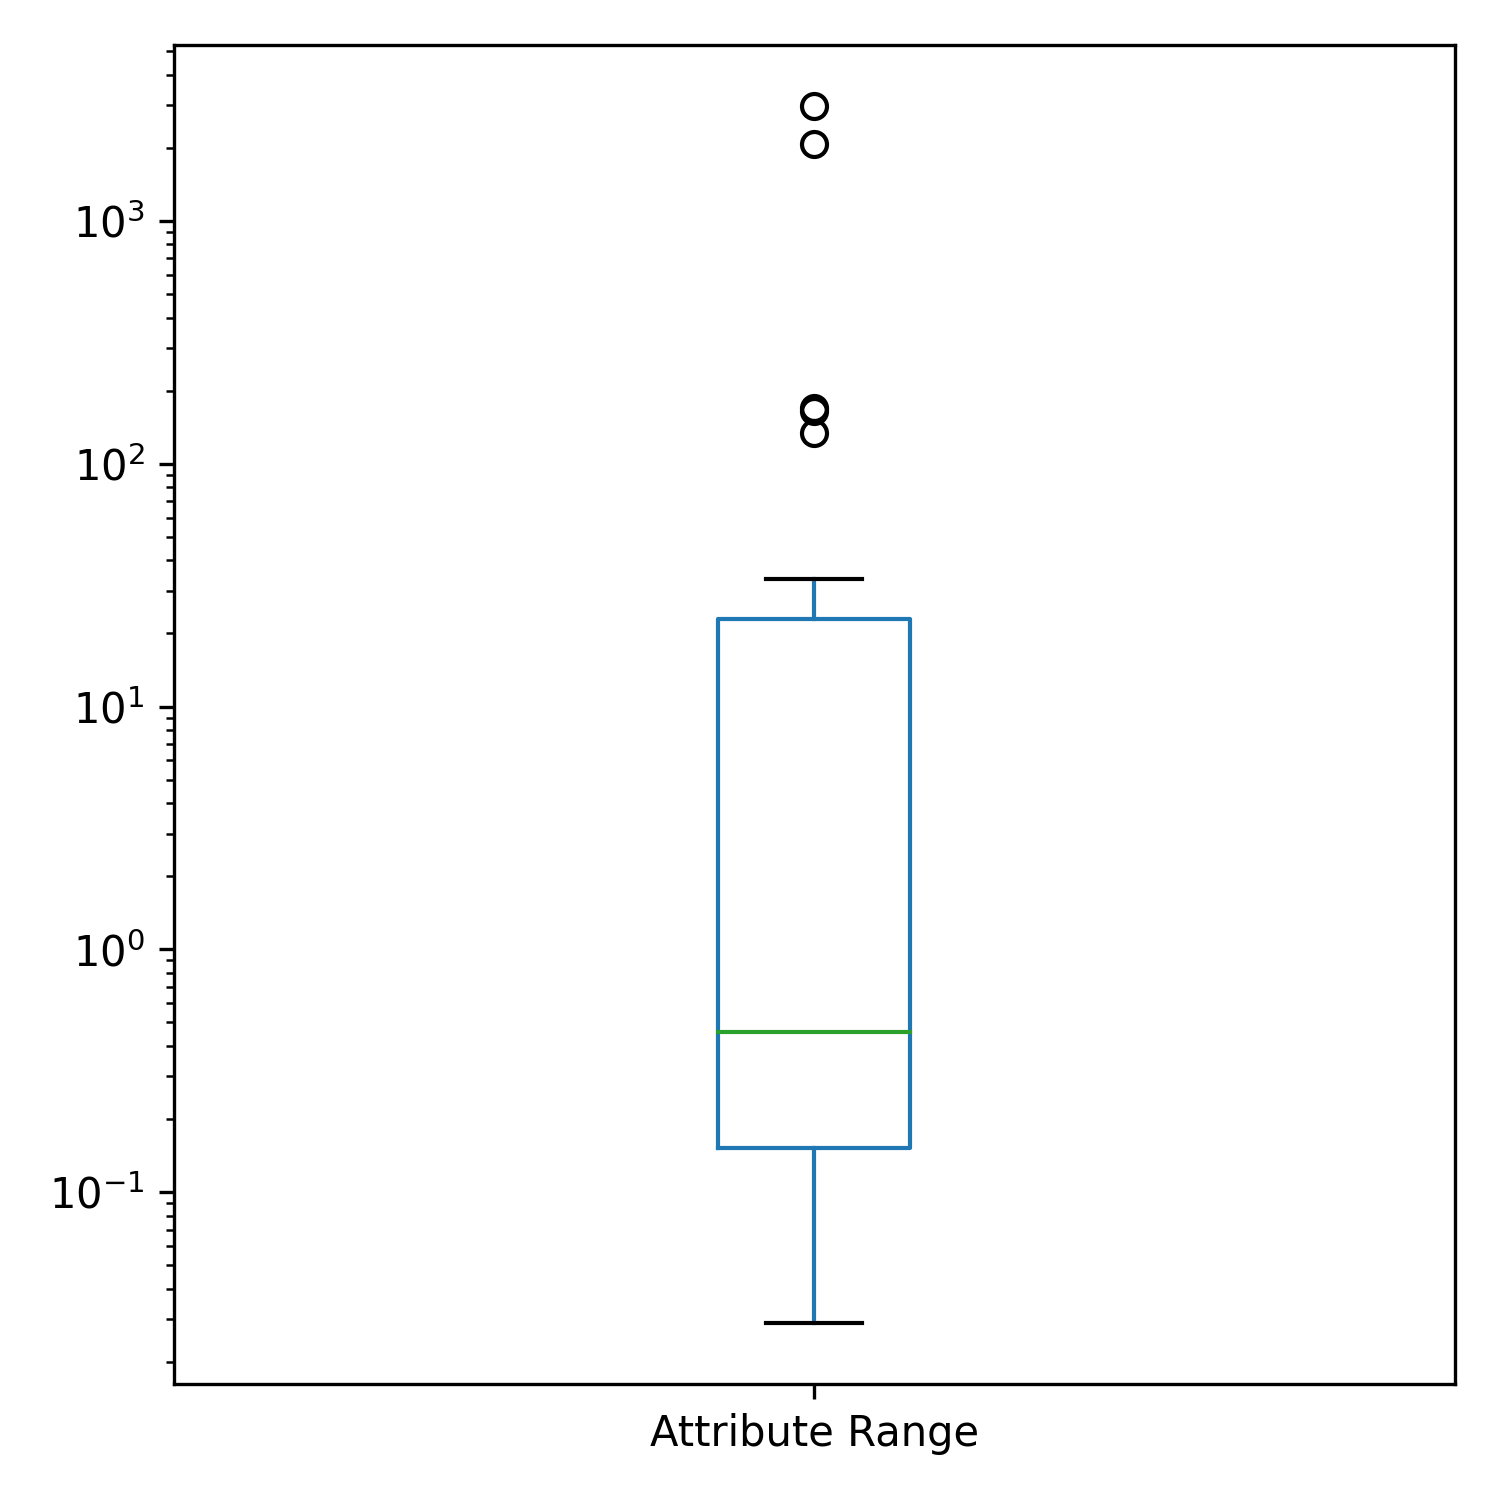
\includegraphics[width=0.9\textwidth]{exercise_1/paper/figures/breast_cancer_range_plot.png}
            \caption{Boxplot of the values ranges of the attributes}
            \label{fig:breast-cancer_value_ranges}
        \end{subfigure}
        \begin{subfigure}[c]{0.45\textwidth}
            \centering
            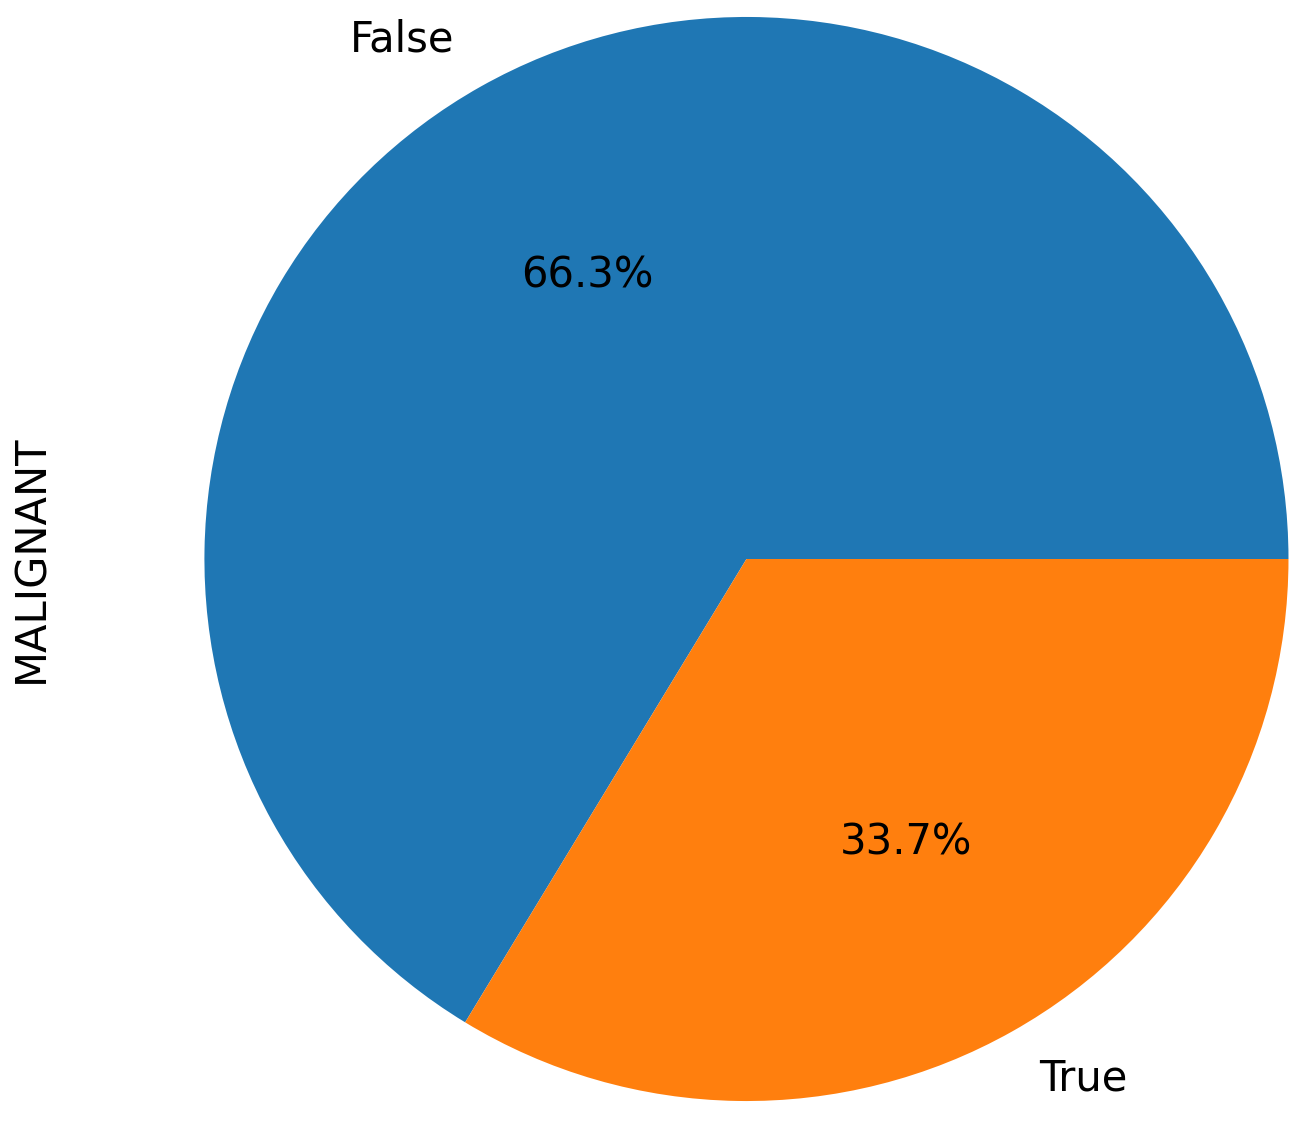
\includegraphics[width=1\textwidth]{figures/breast_cancer_malignant_pie.png}
            \caption{Class distribution}
            \label{fig:breast-cancer_classes_pie}
        \end{subfigure}
        \caption{Figures for the Breast Cancer dataset}
        \label{fig:breast-cancer}
    \end{figure}
    
    The goal of the classification problem is to predict for $284$ patients whether they have a malignant event (true) or not (false) based on the given attributes of the patient. In our dataset the proportion of samples with resp. without a malignant event is about $1:2$ (see Figure~\ref{fig:breast-cancer_classes_pie}).
    
Because of the imbalanced classes and the importance for a patient with breast cancer to be positively classified, we chose recall and accuracy as the performance measures for this dataset. 
    
    \subsection{$k$-NN}
        Since the given dataset has very different value ranges, the first issue we encountered was that we had to scale the attributes because the spread of values was vastly different. In order to eliminate a wrong influence of attributes we normalised them via min-max scaling resp. standard scaling using the built in tools in scikit-learn. 
        
        Afterwards, we built different classifiers using different parameters, e.g. varying $k$ or changing the weight function. We evaluated these classifiers via $5$-fold cross-validation over the given training set. Our tests showed that using scaling yields to a better classifier, but it does not make a difference if the min-max scaler or the standard scaler is used. This was the reason why we did not include the scaling method explicitly in this documentation. Table~\ref{tbl:kNN_breast-cancer_cross-validation} shows some results for the accuracy and recall for different parameter settings of $k$ and the weight function. For each classifier the average performance of accuracy and recall and the respective standard deviation is stated.
        
        \begin{table}[h]
        \centering
            \begin{tabular}[h]{r|c|c|c|c|c|}
                \multirow{2}{*}{$k$} & \multirow{2}{*}{weight} & \multicolumn{2}{|c|}{accuracy} & \multicolumn{2}{|c|}{recall} \\
                & & avg. perform. & std. & avg. perform. & std. \\
                \hline
                $3$ & distance & $0.979$ & $0.013$ & $0.957$ & $0.039$\\
                \hline
                $5$ & distance & $0.982$ & $0.011$ &$0.957$ & $0.039$\\
                \hline
                $5$ & uniform & $0.982$ & $0.011$ & $0.957$ & $0.039$\\
                \hline
                $11$ & uniform & $0.975$ & $0.014$ & $0.927$ & $0.041$ \\
                \hline
                $21$ & uniform & $0.9719$ & $0.0179$ & $0.9168$ & $0.0533$ \\
                \hline
                $51$ & distance & $0.9404$ & $0.0238$ & $0.8342$ & $0.0664$
            \end{tabular}
            \caption{Results of $k$-NN for breast cancer dataset via cross-validation}
            \label{tbl:kNN_breast-cancer_cross-validation}
        \end{table}
        
        One can see that in our split using small values for $k$ yields to better results considering the accuracy or the recall and that using a weight function makes hardly a difference for both performance measures. Also the standard deviation is for both measures very small, which is good. 
        
        The runtime for the classification is $0.002$, so a fraction of a second. Furthermore, we do not need to build a classifier. Hence, this algorithm runs very fast, especially because of the comparatively small $k$ values and the relatively small dataset.
        
        The results for the holdout method can be seen in Table~\ref{tbl:kNN_breast-cancer-holdout}. As we have only one split the standard deviation is for the accuracy as well as the recall always equal to $0$.
        
        \begin{table}[h]
        \centering
            \begin{tabular}[h]{r|c|c|c|c|c|}
               \multirow{2}{*}{$k$} & \multirow{2}{*}{weight} & \multicolumn{2}{|c|}{accuracy} & \multicolumn{2}{|c|}{recall} \\
                & & perform. & std. & perform. & std. \\
                \hline
                $3$ & distance & $0.9444$ & $0.0$ & $0.8519$ & $0.0$ \\
                \hline
                $5$ & distance & $0.9444$ & $0.0$ & $0.851$ & $0.0$ \\
                \hline
                $5$ & uniform & $0.9444$ & $0.0$ & $0.851$ & $0.0$ \\
                \hline
                $11$ & uniform & $0.9444$ & $0.0$ & $0.851$ & $0.0$ \\
                \hline
                $21$ & uniform & $0.9306$ & $0.0$ & $0.815$ & $0.0$ \\
                \hline
                $51$ & distance & $0.9167$ & $0.0$ & $0.778$ & $0.0$
            \end{tabular}
            \caption{Results of $k$-NN for breast cancer dataset via holdout}
            \label{tbl:kNN_breast-cancer-holdout}
        \end{table} 
        
        Via the holdout method we obtained similar results for different parameter settings. Thus, one could conclude that the algorithm is not sensitive to different parameter settings. But this must not be necessarily true as the holdout method tests only on one split. As we have seen in the cross-validation method varying the parameters did change the optimality of the classifier, but the differences were not very big. 
        
        Because the standard value of $k=5$ performed best in our cross-validation tests and was also one of the best values in the holdout method, we used it for the Kaggle competition. Using $k=5$ with uniform weights we received a $1.0$ score on the public leaderboard. We also tried different values for $k$ and used the distance as weight function but could obviously could not obtain a better value than the perfect score as for $k=5$, which was consistent with the results above.
    
    \subsection{Decision Tree}
        In this algorithm scaling is not needed as we do not need to measure the distance between samples. For building a decision tree we can change multiple parameters, e.g. the maximum depth of the tree or the criterion to measure the quality of a split which could be 'gini' or 'entropy'.
        
        \begin{table}[h!]
            \centering
            \begin{tabular}[h]{l|c|c|c|c|c|}
                \multirow{2}{*}{criterion} & \multirow{2}{*}{max. depth} & \multicolumn{2}{|c|}{accuracy} & \multicolumn{2}{|c|}{recall} \\
                & & avg. perform. & std. & avg. perform. & std. \\
                \hline
                entropy &$4$ & $0.951$ & $0.034$ &$0.937$ & $0.051$\\
                \hline
                gini & $5$ & $0.975$ & $0.014$ & $0.937$ & $0.077$\\\hline
                entropy & $5$ & $0.954$ & $0.017$ & $0.907$ &$0.081$\\\hline
                gini & $8$ & $0.958$  & $0.029$ & $0.969$ & $0.025$\\
                \hline
                entropy & $9$ & $0.958$ & $0.029$ & $0.958$ & $0.039$\\
                \hline
                gini & $9$ & $0.964$ & $0.025$ & $0.937$ & $0.077$
            \end{tabular}
            \caption{Results of decision tree for breast cancer dataset via cross-validation}
            \label{tbl:decision-tree_breast-cancer_cross-validation}
        \end{table}
        Table~\ref{tbl:decision-tree_breast-cancer_cross-validation} shows the average performance of accuracy and recall with the respective standard deviations of some of the parameter settings evaluated via cross-validation. 
        From these tests we can conclude the following. Considering the accuracy 'gini' performed for different tree lengths better as a splitting criterion than 'entropy', whereby performing best for a maximum depth of $5$. Measuring the recall both criterion performed rather similarly, with the best recall value being for 'gini' and a maximum depth of $8$. It should be noted that considering the recall 'gini' is not always better than 'entropy'. Hence, we can not state optimal parameter settings like for $k$-NN, since the standard deviations for the respective settings are comparatively small. 

        We also evaluated the decision trees using the holdout method. Table~\ref{tbl:decision-tree_breast-cancer_holdout} shows the results. Like for the previous algorithm the standard deviation is equal to $0$ for both performance measures as we are only considering one split of the data. Hence, we did not include it in the table.
        
        \begin{table}[h!]
            \centering
            \begin{tabular}[h]{l|c|c|c|}
                criterion & max. depth & accuracy & recall \\
                \hline
                entropy &$4$ & $0.958$ & $0.889$\\
                \hline
                gini & $5$ & $0.958$ & $0.926$\\\hline
                entropy & $5$ & $1$ & $1$\\\hline
                gini & $8$ & $0.958$ & $0.963$\\
                \hline
                entropy & $9$ & $0.972$ & $0.926$\\
                \hline
                gini & $9$ & $0.972$ & $0.926$\\
            \end{tabular}
            \caption{Results of decision tree for the breast cancer dataset via holdout}
            \label{tbl:decision-tree_breast-cancer_holdout}
        \end{table}
        
        We can see that the holdout method returned a perfect classifier with full accuracy and recall for the corresponding split with 'entropy' as criterion a maximum depth of $5$. Compared with the results of cross-validation this was not one of the optimal settings. For this method 'entropy' performed in general a bit better than 'gini' resp.\ not worse. 
        
        Since the holdout method evaluates only on one training/test split, the results depend only on the quality of this single split. Via cross-validation we train using multiple splits, whereby we can balance the quality. This is the reason why we will document only the results obtained by cross-validation for the following classifiers resp.\ datasets. However, we will remark major differences between these two methods, if we observe any.
        
        After these tests we can see that on the given dataset changing different parameter settings in the decision tree algorithm did change the scores of the classifier, but the differences were not really big. However, there were apparent differences between the holdout and the cross-validation testing. Considering the results of cross-validation, as this is less dependent of the quality of one single split, the differences of accuracy resp. recall is rather small. Hence, we can conclude that it is not very sensitive to different parameter settings for this dataset.
        
        Using the best parameter settings of our testing we submitted it to the Kaggle competition. However, the best score on the public leaderboard was still worse than the results from $k$-NN. We reasoned that the cause for the comparatively bad results in Kaggle was that $k$-NN was simply better suited for this dataset. 
        
        %Not limiting the depth of the decision tree gave us a depth of $7$ on the learning set, which is not high considering the dimension of $32$ and the size of the test set. Therefore, we did not limit the depth of the decision tree as it did not seem to be overfitted. Since the first result was only $0.92307$, which compared to the $k$-NN classifier was quite bad we decided to set the splitter to random to see whether the results changed. The result was slightly better but that might have been luck rather than an actually better tree. Using the entropy instead of the gini impurity to measure the quality of a split, we obtained slightly better results, but there was still room for improvement.
        
%    \subsection{Perceptron}
%       Surprisingly the perceptron classifier performed well on the public leaderboard giving a score of $1.0$ like $k$-NN at the first try. Changing the maximum number of iterations as well as $\alpha$ did not change the result of the perceptron, which implied that the perceptron converged to a stable state.
    
    \subsection{Random Forest}
        Changing the parameter values described in Section~\ref{subsec:random-forest} provided a lot of information. We decided to document the results of accuracy and recall for different numbers of trees and weights associated with the classes, which can be seen in Figure~\ref{fig:breast-cancer_random-forest}. For the other parameters in the algorithm we considered the default values. 
        
        \begin{figure}[h!]
            \centering
            \begin{subfigure}[c]{0.45\textwidth}
                \centering
                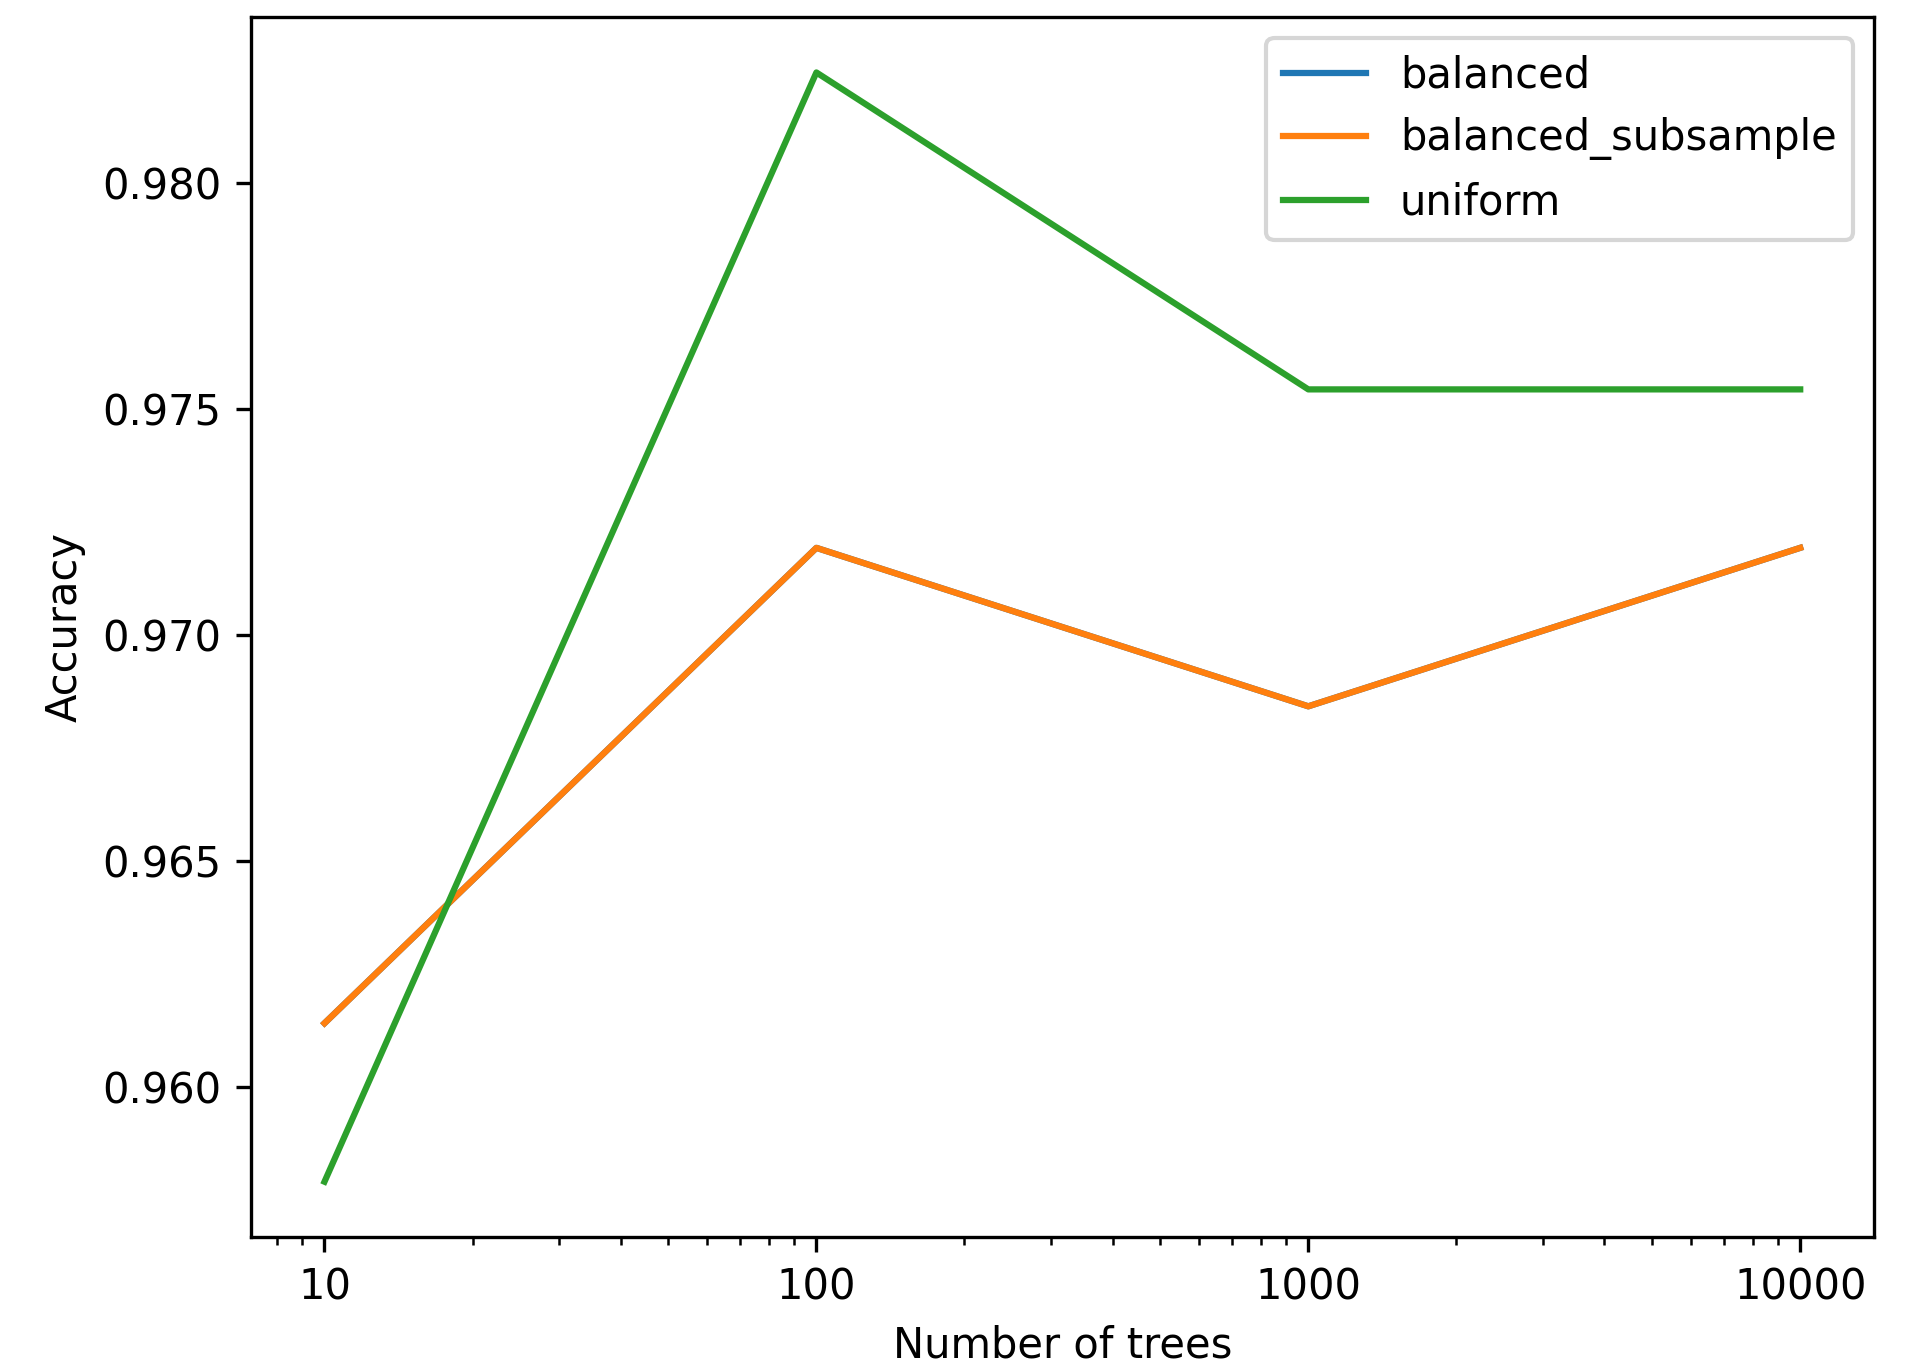
\includegraphics[width=1\textwidth]{exercise_1/paper/figures/breast-cancer-accuracy-random_forest.png}
                \caption{Accuracy}
                \label{fig:breast-cancer_random-forest_accuracy}
            \end{subfigure}
            \begin{subfigure}[c]{0.45\textwidth}
                \centering
                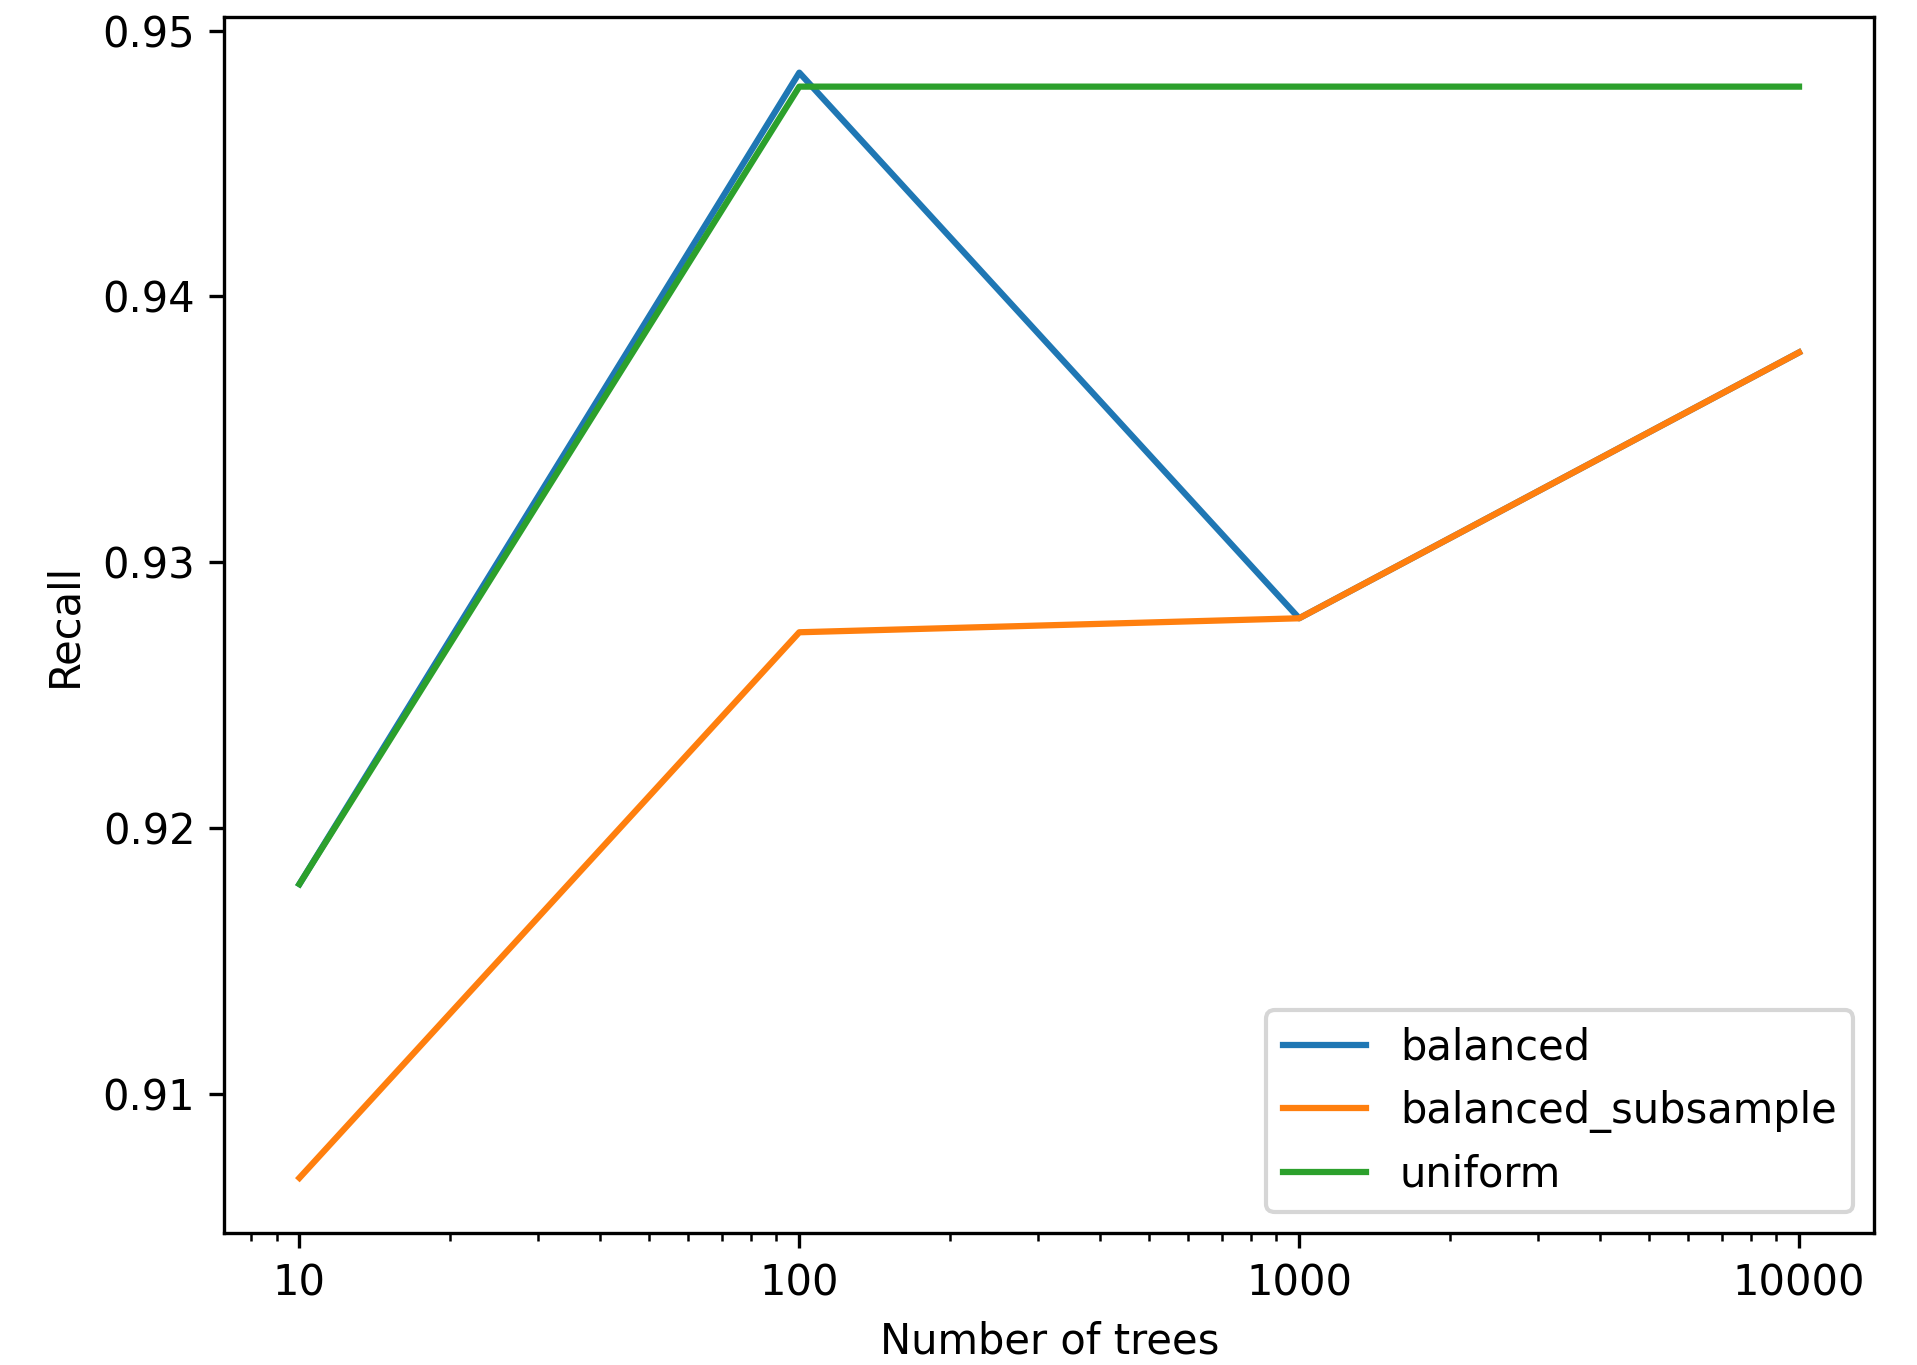
\includegraphics[width=1\textwidth]{exercise_1/paper/figures/breast-cancer-recall-random_forest.png}
                \caption{Recall}
                \label{fig:breast-cancer_random-forest_recall}
            \end{subfigure}
            \caption{Performance measures of random forest for breast cancer dataset}
            \label{fig:breast-cancer_random-forest}
        \end{figure}
        
        In Figure~\ref{fig:breast-cancer_random-forest_accuracy} the performance of 'balanced' and 'balanced\_subsample' is almost identical, independent of the number of trees. The difference between these two settings is that the weights are computed based on the bootstrap sample for every tree grown and not on the whole dataset. Additionally, one can see that uniform weights performed the best, except for a small number of trees, with a peek at $100$ trees. 
        
        The recall however improved with a higher number of trees for 'uniform' and 'balanced\_subsample' class weights. Whereas with a 'balanced' class weight the measure decreased between a number of $100$ and $1\,000$ trees, which can be seen in Figure~\ref{fig:breast-cancer_random-forest_recall}.
        
        For this algorithm we did a parameter search on the random forest algorithm for the number of trees, the maximum depth of the tree, the criterion to measure the quality of a split and some other parameters. We obtained the following: 
        \begin{itemize}
            \item Number of trees: $10\,000$
            \item Maximum depth of a tree: None
            \item Minimum number of samples required to split an internal node: $5$
            \item Minimum number of samples required to be at a leaf node: $1$
            \item Number of features to consider when looking for the best split: 'sqrt'
            \item Bootstrap samples are used when building tree: False
            \item Weights associated with classes: 'balanced\_subsample'
        \end{itemize}
        
        The obtained parameters were interesting because of various aspects. First, the treedepth was unlimited, which one would expect to be a possible cause of overfitting. Second, bootstrapping the samples for tree generation was turned off and as class weight 'balanced\_subsample' was used, which is interesting, since this class weight function calculates the weights inversly proportional to the class frequencies in the input data, but based on the subsample of a bootstrapped tree. As the trees are not bootstrapped every feature is used for every tree generation and therefore 'balanced\_subsample' should be equal to 'balanced'. We suspect that it actually is, but share the first place on the parameter search, so only one of those parameter options is returned.

        Next, we submitted the classifier learned with the obtained parameters to the Kaggle competition which resulted in a score of $0.96$ on the public test set. This was pretty good, especially compared with the decision tree approach. However, it was still not as good as the the $k$-NN classifier.
        
        As stated in Section~\ref{subsec:random-forest} a big disadvantage of this algorithm is its runtime. Compared with $k$-NN and decision tree, which have a runtime of at most few seconds, this algorithm needs about $20$ seconds to compute the best classifier with $10\,000$ trees. 
    
\section{Amazon Commerce Reviews}
    For this problem a dataset with $10\,000$ numeric attributes with integer values was given. Figure~\ref{fig:amazon_value_ranges} shows a boxplot diagramm of the value ranges of the attributes of the $749$ samples in the dataset. It can be seen that the range of most of the features is less than 10, but we also have some attributes with a big range. 
    
    \begin{figure}[h!]
        \centering
        \begin{subfigure}[c]{0.45\textwidth}
            \centering
            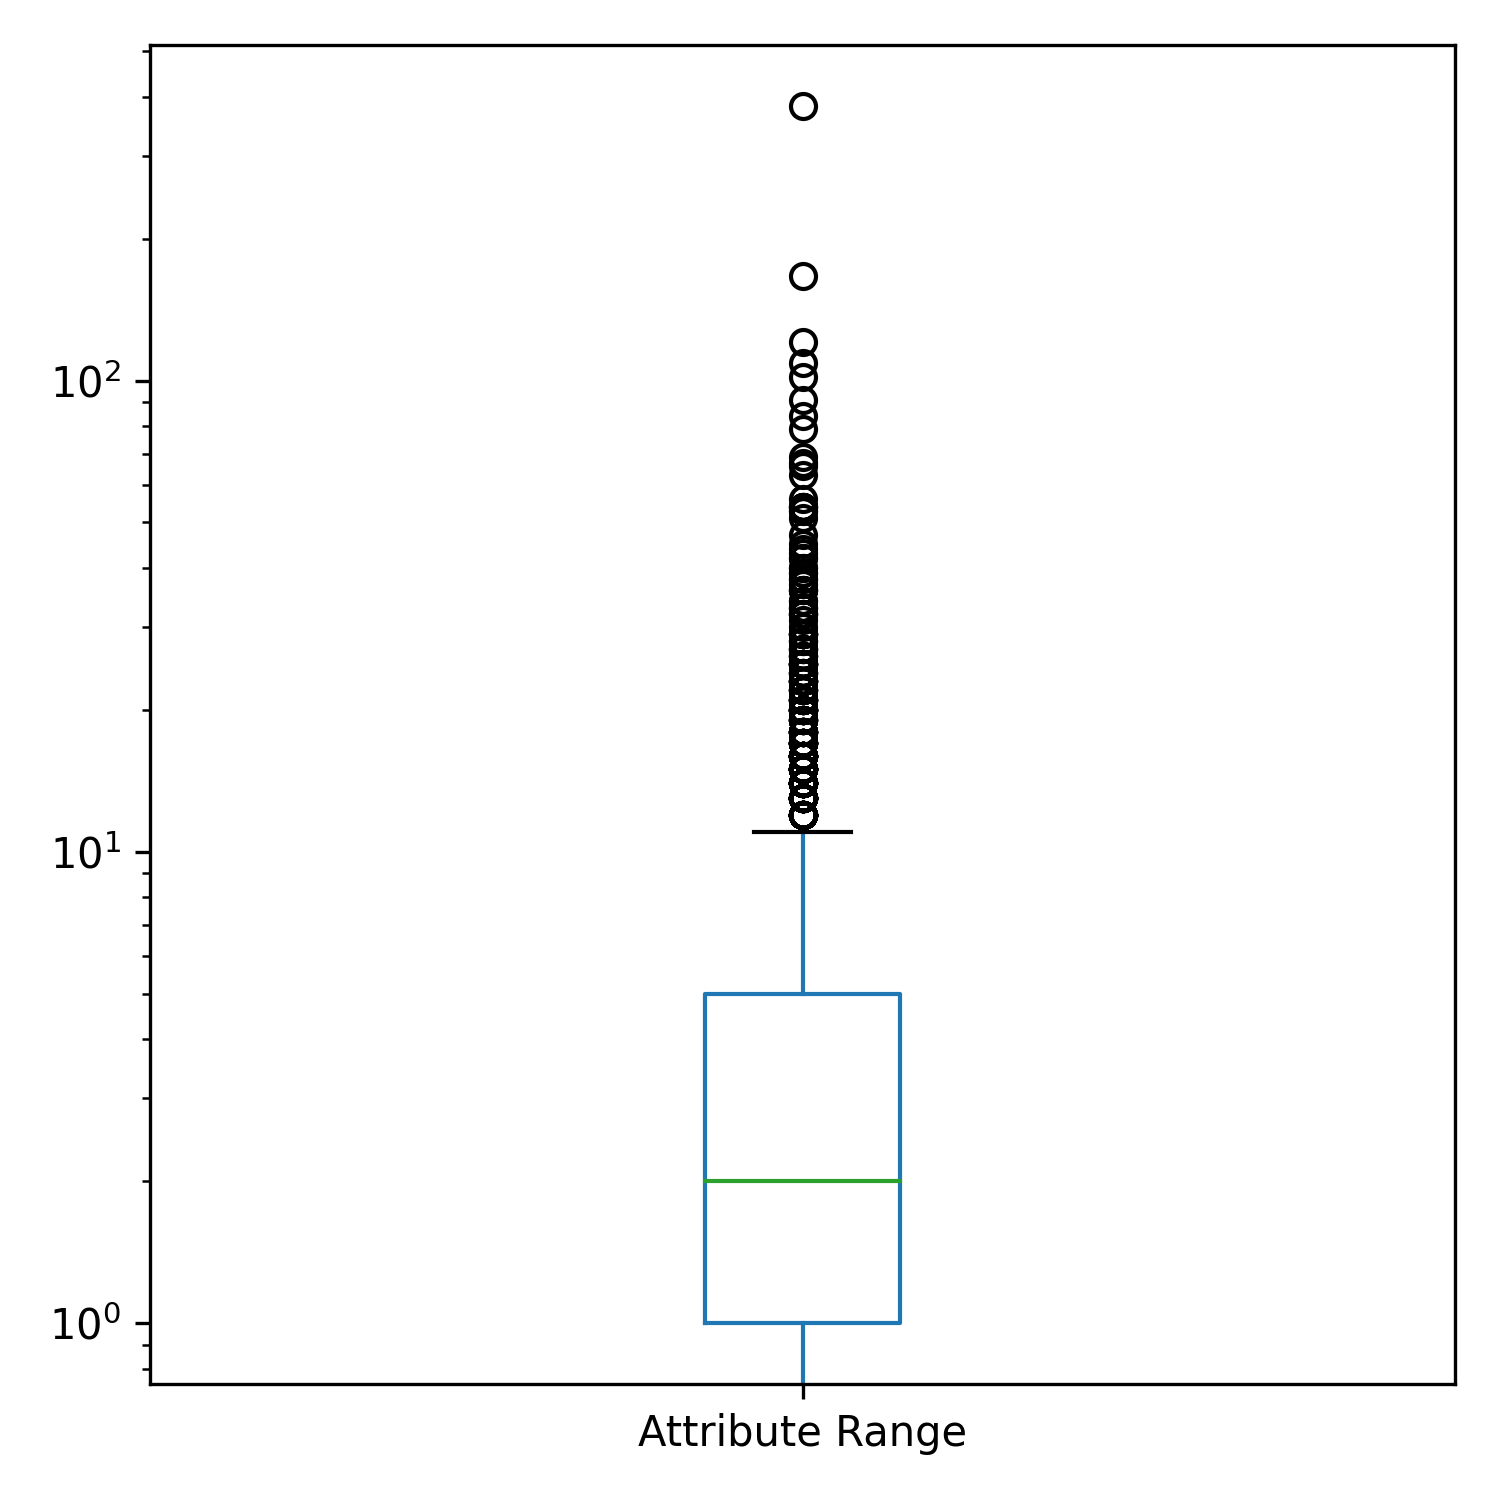
\includegraphics[width=1\textwidth]{exercise_1/paper/figures/amazon_classes_range_plot.png}
            \caption{Boxplot of the values ranges of the attributes}
            \label{fig:amazon_value_ranges}
        \end{subfigure}
        \begin{subfigure}[c]{0.45\textwidth}
            \centering
            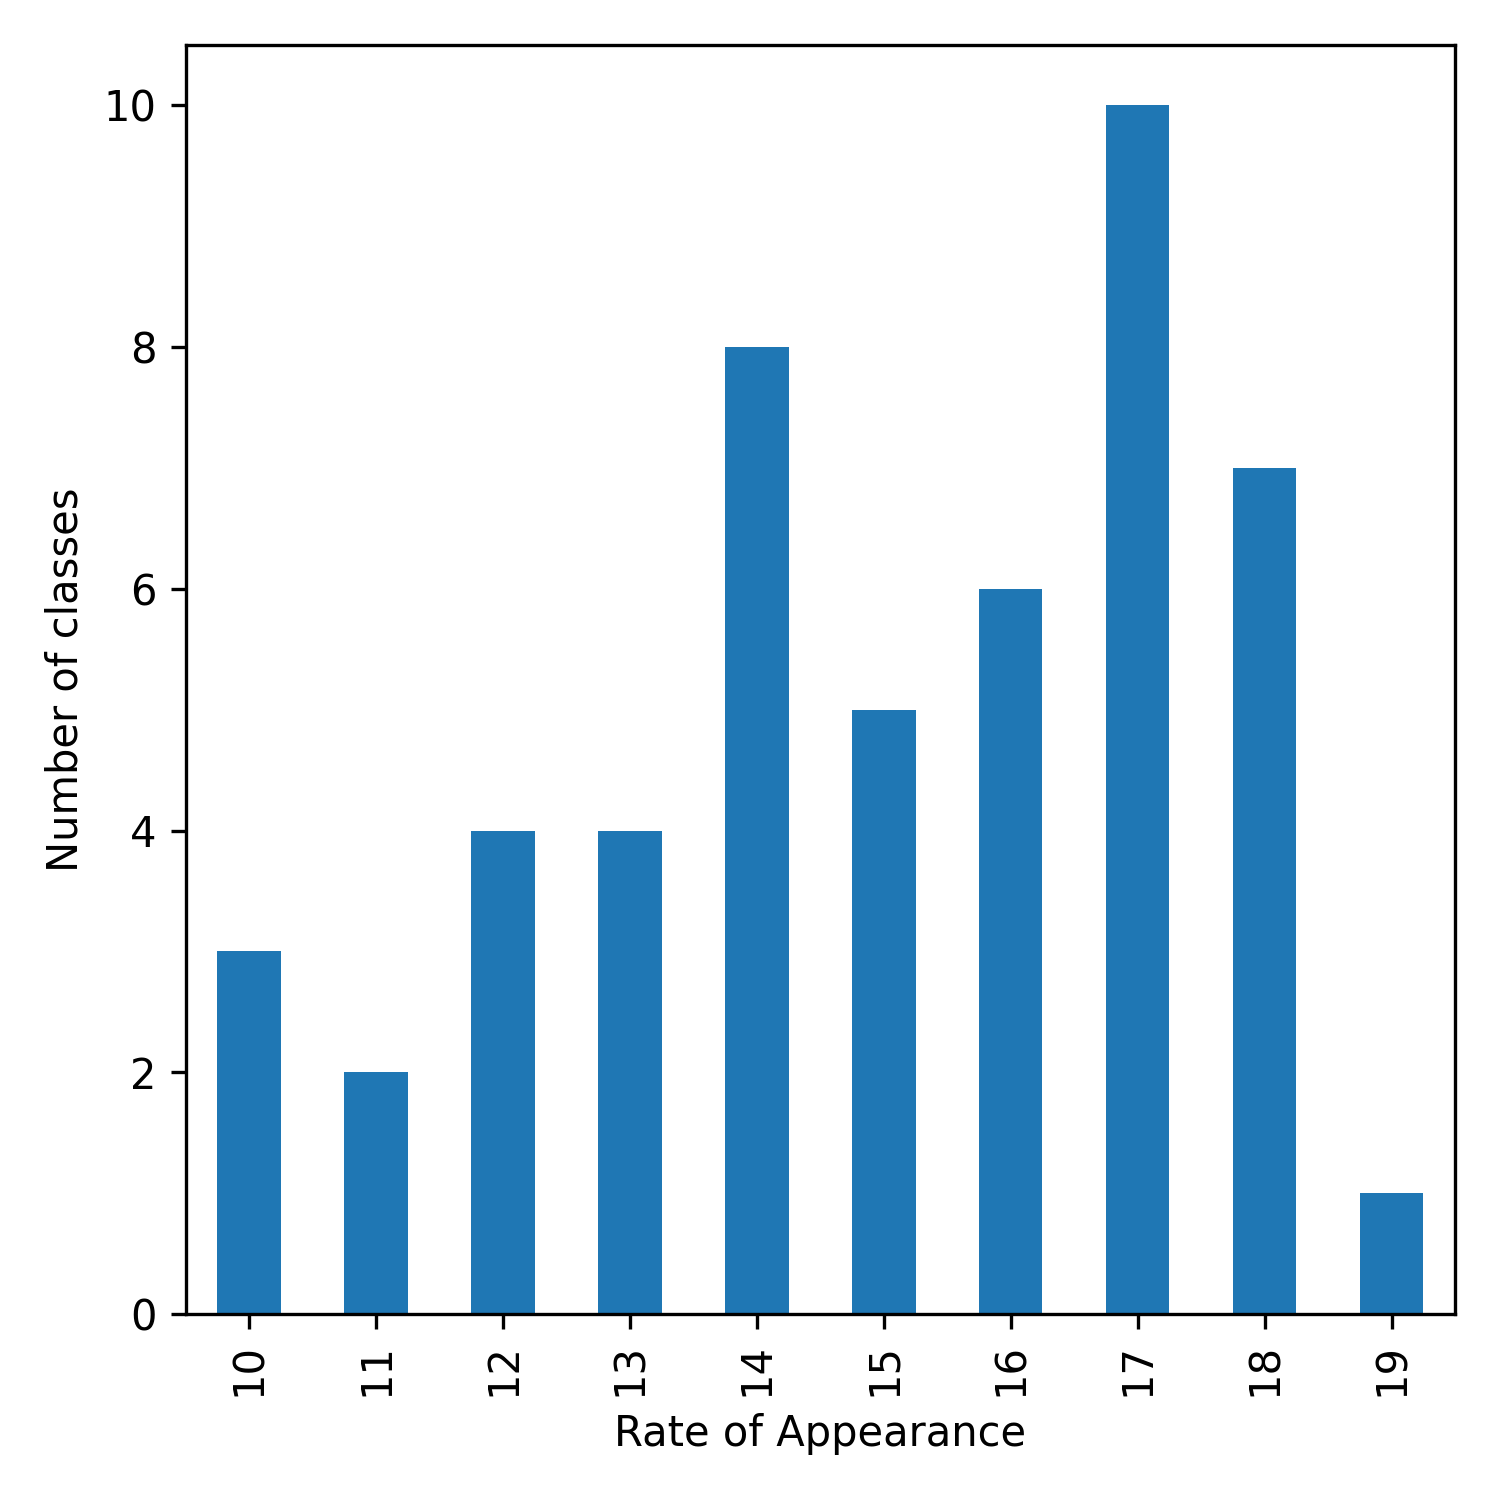
\includegraphics[width=1\textwidth]{figures/amazon_classes_bar.png}
            \caption{Class distribution}
            \label{fig:amazon_classes_bar}
        \end{subfigure}
        \caption{Figures for the Amazon Commerce Review dataset}
        \label{fig:amazon}
    \end{figure}
    
    Based on these attributes the aim was to predict a nominal feature with $50$ possible values, namely who submitted a review. The distribution of the classes is not uniform, as this would mean that for each class there are about $15$ samples in our dataset which is not the case. Figure~\ref{fig:amazon_classes_bar} shows on the $x$-axis the number of samples in a class and on the $y$-axis the number of classes with the corresponding number of samples, e.g. there are 3 classes, each with 10 samples of the dataset. It can be seen that the distribution is not uniform and about half of the classes have a sample size per class between $16$ and $18$.
    
    Because we do not have a binary decision problem, the performance measures recall and precision are rather meaningless. One could look at the accuracy per class, but as the classes were all roughly the same size we decided to forgo this.

    \subsection{$k$-NN}
        For this dataset we first learned some classifiers and submitted it to the Kaggle competition before evaluating it locally on the given dataset.
        
        We run the $k$-NN algorithm with different values for $k$. 
        First, we normalised the data using the min-max-scaling and tried $k=5$, since this was the default value in scikit-learn, which led to a very good result in the Breast Cancer dataset. Unfortunately, we obtained a very bad result of $0.05$. Our next attempts with higher values for $k$ did not yield to an improvement. Finally, we tried $k=1$ which improved the result to $0.12$.
        
        Next, we submitted a classifier trained on the original data, i.e. without scaling the variables and setting the distance as weight function. With these setting we obtained better scores, namely $0.216$ for $k=1$ and $0.267$ for $k=5$. 
        
        Apparently, we could not obtain good results with this approach since the number of submissions per day was limited. Hence, we tried to find optimal parameter values locally before submitting it to the competition. Again, we evaluated different classifiers via cross-validation resp.\ the holdout method. Table~\ref{tbl:kNN_amazon_cross-validation} shows the results of $k$-NN classifiers using some different settings for $k$, the weight function and the scaling method.
        
        \begin{table}[h!]
        \centering
            \begin{tabular}[h]{r|c|c|c|c}
                $k$ & weight & scaling & avg. accuracy & std.\\
                \hline
                $1$ & arbitrary & no & $0.2667$ & $0.0337$ \\
                \hline
                $1$ & arbitrary & min-max & $0.1227$ & $0.0275$ \\
                \hline
                $3$ & uniform & min-max & $0.0747$ & $0.0122$ \\
                \hline
                $3$ & distance & standard & $0.0653$ & $0.154$ \\
                \hline
                $5$ & distance & no & $0.2507$ & $0.326$ \\
                \hline
                $5$ & distance & min-max & $0.1013$ & $0.0195$ \\
                \hline
                $11$ & uniform & standard & $0.0293$ & $0.0068$ \\
                \hline
                $11$ & uniform & no & $0.2093$ & $0.0108$
            \end{tabular}
            \caption{Results of $k$-NN for Amazon reviews dataset via cross-validation}
            \label{tbl:kNN_amazon_cross-validation}
        \end{table}
        
        One can see that the difference between the min-max scaler and the standard scaler is rather small. Whereas without scaling the obtained classifiers are much better, even for different $k$ values. From our tests we can conclude that without scaling the attributes, considering the first nearest neighbor is the best prediction we can make with the $k$-NN algorithm. Nevertheless, with an accuracy of $0.2667$ this is still not good enough. 
        
        The average runtime of this algorithm is about $1$ second, which is very fast but compared with the breast cancer dataset much slower. The reason behind this is the size of the dataset and the number of attributes as both of these numbers are higher compared to the breast cancer dataset. 
        %avg runtime: $1.0795$ seconds
        
        Although we tried different parameters for this algorithm, the classifiers still performed poorly. We think the reason for this is because of the high number of attributes and a comparatively low number of samples.
        
    %\subsection{Perceptron}
      %  Another approach was using a multilayer perceptron. The resulting classifier performed only slightly better than $k$-NN with a score of about $0.075$.
       % We think that the test data is not linear separable, and therefore a simple perceptron is not the way to go.
        %\todo[inline]{Reasoning: same as above?}
        %\todo[inline]{different parameters like max number of iterations or alpha?}
        
    \subsection{Decision Tree}
        As we could change many different parameters to obtain a better classifier, we decided to split our data first and then evaluate the classifiers on the test set before submitting it to the Kaggle competition. The results of the cross-validation method with different parameter settings can be seen in Table~\ref{tbl:decision-tree_amazon_cross-validation}. Furthermore, this algorithm had an average running time of $2.2$ seconds, which is slower than $k$-NN. 
    
        %A decision tree with unbounded depth and the default values of scikit-learn instantly performed better than the default values of $k$-NN with a score of $0.189$. Limiting the maximal depth however did not yield to greatly different results.
        
        %As we could change many different parameters to obtain a better classifier, we decided to split our data into a $75\%$ training and $25\%$ test set and evaluate the classifiers first on the test set before submitting it to the Kaggle competition. The results of this holdout method can be seen in Table~\ref{tbl:decision-tree_amazon}. Additionally, we also tested different parameters classifiers via cross-validation, where the results can also be seen in Table~\ref{tbl:decision-tree_amazon_cross-validation}.
        
        \begin{table}[h!]
            \centering
            \begin{tabular}[h]{l|c|c|c}
                criterion & max. depth & avg. accuracy & std. \\
                \hline
                gini & 5 & $0.124$ & $0.009$ \\
                \hline
                entropy & 7 & $0.2053$ & $0.0351$ \\
                \hline
                gini & 7 & $0.1467$ & $0.0112$ \\
                \hline
                gini & 11 & $0.2173$ & $0.0371$ \\
                \hline
                entropy & 11 & $0.204$ & $0.0209$ \\
                \hline
                entropy & 17 & $0.1907$ & $0.0241$
            \end{tabular}
            \caption{Results of decision tree for Amazon reviews dataset via cross-validation}
            \label{tbl:decision-tree_amazon_cross-validation}
        \end{table}
        
        In general, 'entropy' performed better than 'gini' as criterion but the standard deviation was also a bit higher. Also limiting the maximum depth of the tree resulted in a better classifier.
        
        Based on these results, we picked a few parameter setting and submitted the corresponding classifiers to Kaggle. But we did not expect to get a great score which was the case, as also our evaluation did not yield a good result. Hence, we decided to focus on a random forest instead.
        
    \subsection{Random Forest}
        Using the random forest algorithm for training the classifier turned out to be a lot more successful than our previous attempts. 
        
        %First, we trained $10\,000$ trees and got a result of $0.752$ in the public leaderboard. A big leap in quality. Our tests showed that using 'gini' to measure the quality of a split yielded better results than 'entropy'. That is why we only considered 'gini' as criterion. 
        
        We still tested the classifiers locally on the given training set. Our tests showed that using 'gini' to measure the quality of a split yielded better results than 'entropy'. That is why we only considered 'gini' as criterion. Also a high number of trees improved the classifier. We were optimistic that this algorithm would return a better classifier than $k$-NN and decision tree, as the best obtained accuracy was $0.7227$. 
        
        After some tests we did a parameter search on the number of trees, tree depth and some more parameters of the random forest algorithm. From this we obtained the following values:
        \begin{itemize}
            \item Number of trees: $10\,000$
            \item Maximum depth of a tree: $50$
            \item Minimum number of samples required to split an internal node: $5$
            \item Minimum number of samples required to be at a leaf node: $1$
            \item Number of features to consider when looking for the best split: 'sqrt'
            \item Bootstrap samples are used when building tree: False
        \end{itemize}
        
        The trained classifier with these parameters obtained a score of $0.755$ in the Kaggle competition. Since the distribution of classes is not uniform in the given dataset, we also tried assigning weights to the classes dependent on the class frequencies. This yielded a slightly better result of $0.757$, but as this is the score only for the public test set in Kaggle, we cannot say for sure that it is really an improvement.
        
        A disadvantage of this algorithm is its runtime since this increases noticeably with the number of trees, e.g. for $3\,000$ trees the running time is about $40$ seconds.

\section{Spambase}
    This dataset contains various information about mails, e.g.\ the frequency of words or capital letters, the length of sequences of capital letters in the mail and the appearence of specific words. All of the given attributes are integer or real values. Figure~\ref{fig:spambase_value_ranges} shows a boxplot diagram of the value ranges of all attributes in the Spambase dataset. We can see that the median is 10 but the value ranges vary a lot as we also have outliers with a range of more than $10\,000$. There are no missing values and with a sample size of about $4\,600$ and $58$ attributes this is a rather large and high dimensional dataset compared to the following dataset Credit Approval.
    
    The task is to classify a certain mail as spam (true) or not spam (false) based on the given features. The distribution of the two possible classes of this dataset is shown in Figure~\ref{fig:spambase_classes_pie}. 
    
    \begin{figure}[h!]
        \centering
        \begin{subfigure}[c]{0.45\textwidth}
            \centering
            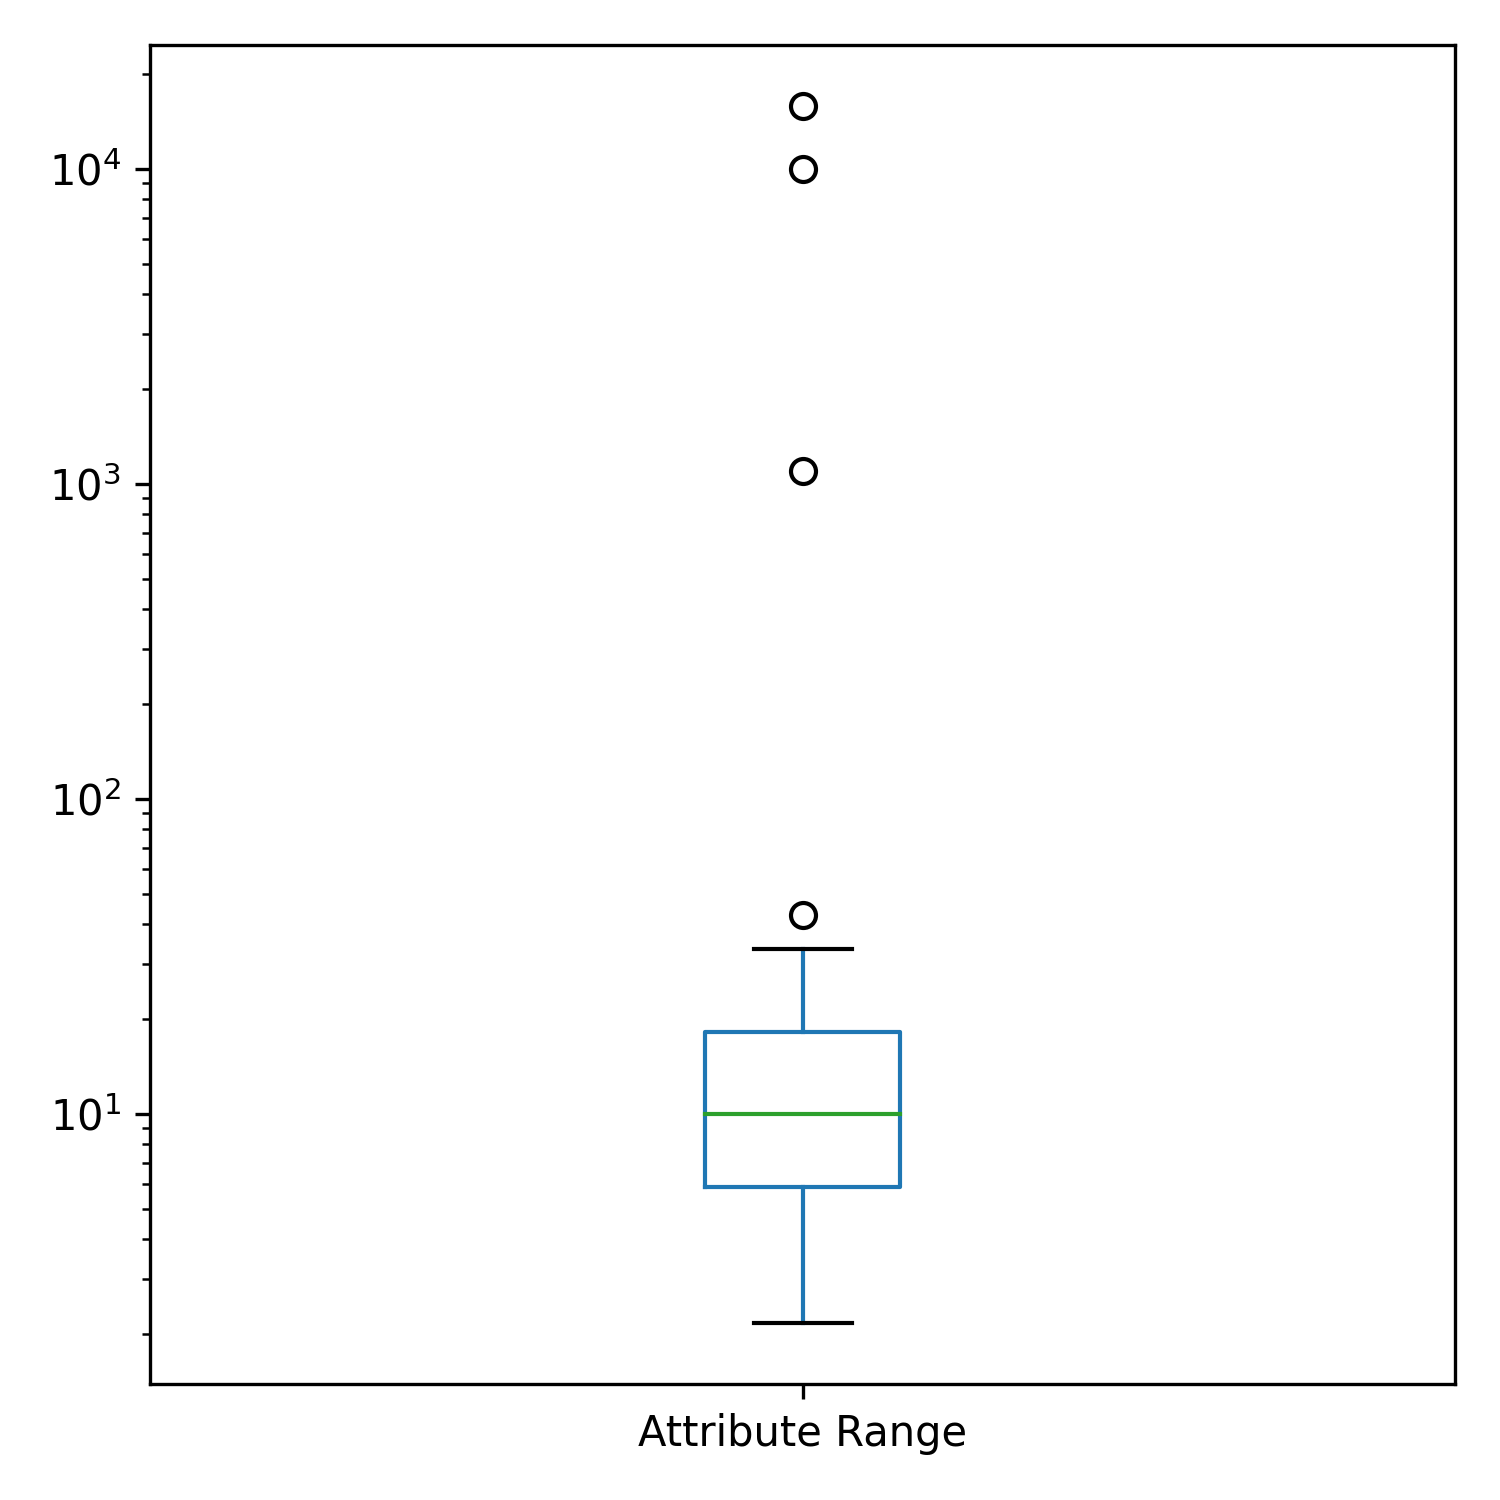
\includegraphics[width=1\textwidth]{figures/spambase_range_plot.png}
            \caption{Boxplot of the values ranges of the attributes}
            \label{fig:spambase_value_ranges}
        \end{subfigure}
        \begin{subfigure}[c]{0.45\textwidth}
            \centering
            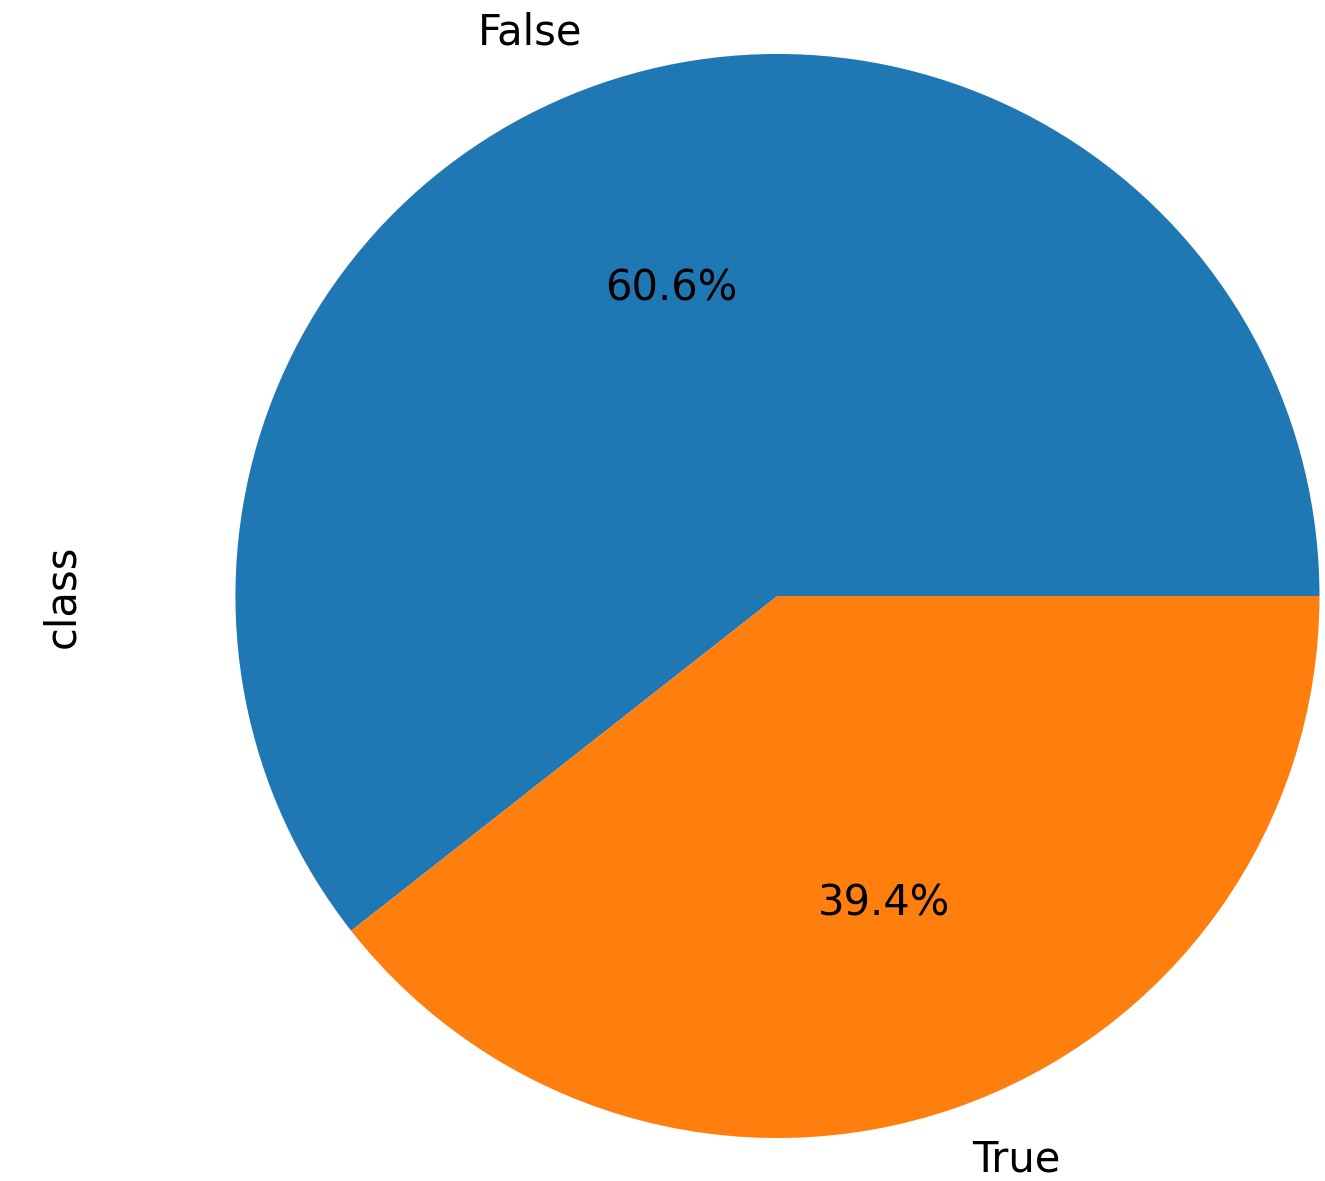
\includegraphics[width=1.1\textwidth]{exercise_1/paper/figures/spambase_positive_pie.png}
            \caption{Class distribution}
            \label{fig:spambase_classes_pie}
        \end{subfigure}
        \caption{Figures for the Spambase dataset}
        \label{fig:spambase}
    \end{figure}
    
    
    \subsection{$k$-NN}
        In Figure~\ref{fig:k-NN_spambase} we have compiled two graphs describing how growing $k$ values and different weight functions affect the average performance of $k$-NN, testing it via cross-validation.
        
        As one can see in the Figures~\ref{fig:k-NN_spambase_accurracy} and \ref{fig:k-NN_spambase_precision} the parameters affect precision and accuracy very differently. While the precision steadily grows for both weight functions with increasing $k$, the accuracy for uniform weights decreases for bigger $k$ values strongly starting at $k\approx 15$. In general distance based weights improve accuracy and precision and are less effected by growing $k$ values.
        The stronger drop of uniform weights makes sense, since far away points might skew the results. The reason for rising precision with rising $k$ could be that all the instances that are classified as spam are grouped closely together while the instances not classified as spam are spread farther in the distance.
        
        \begin{figure}[h!]
            \centering
            \begin{subfigure}[c]{0.45\textwidth}
                \centering
                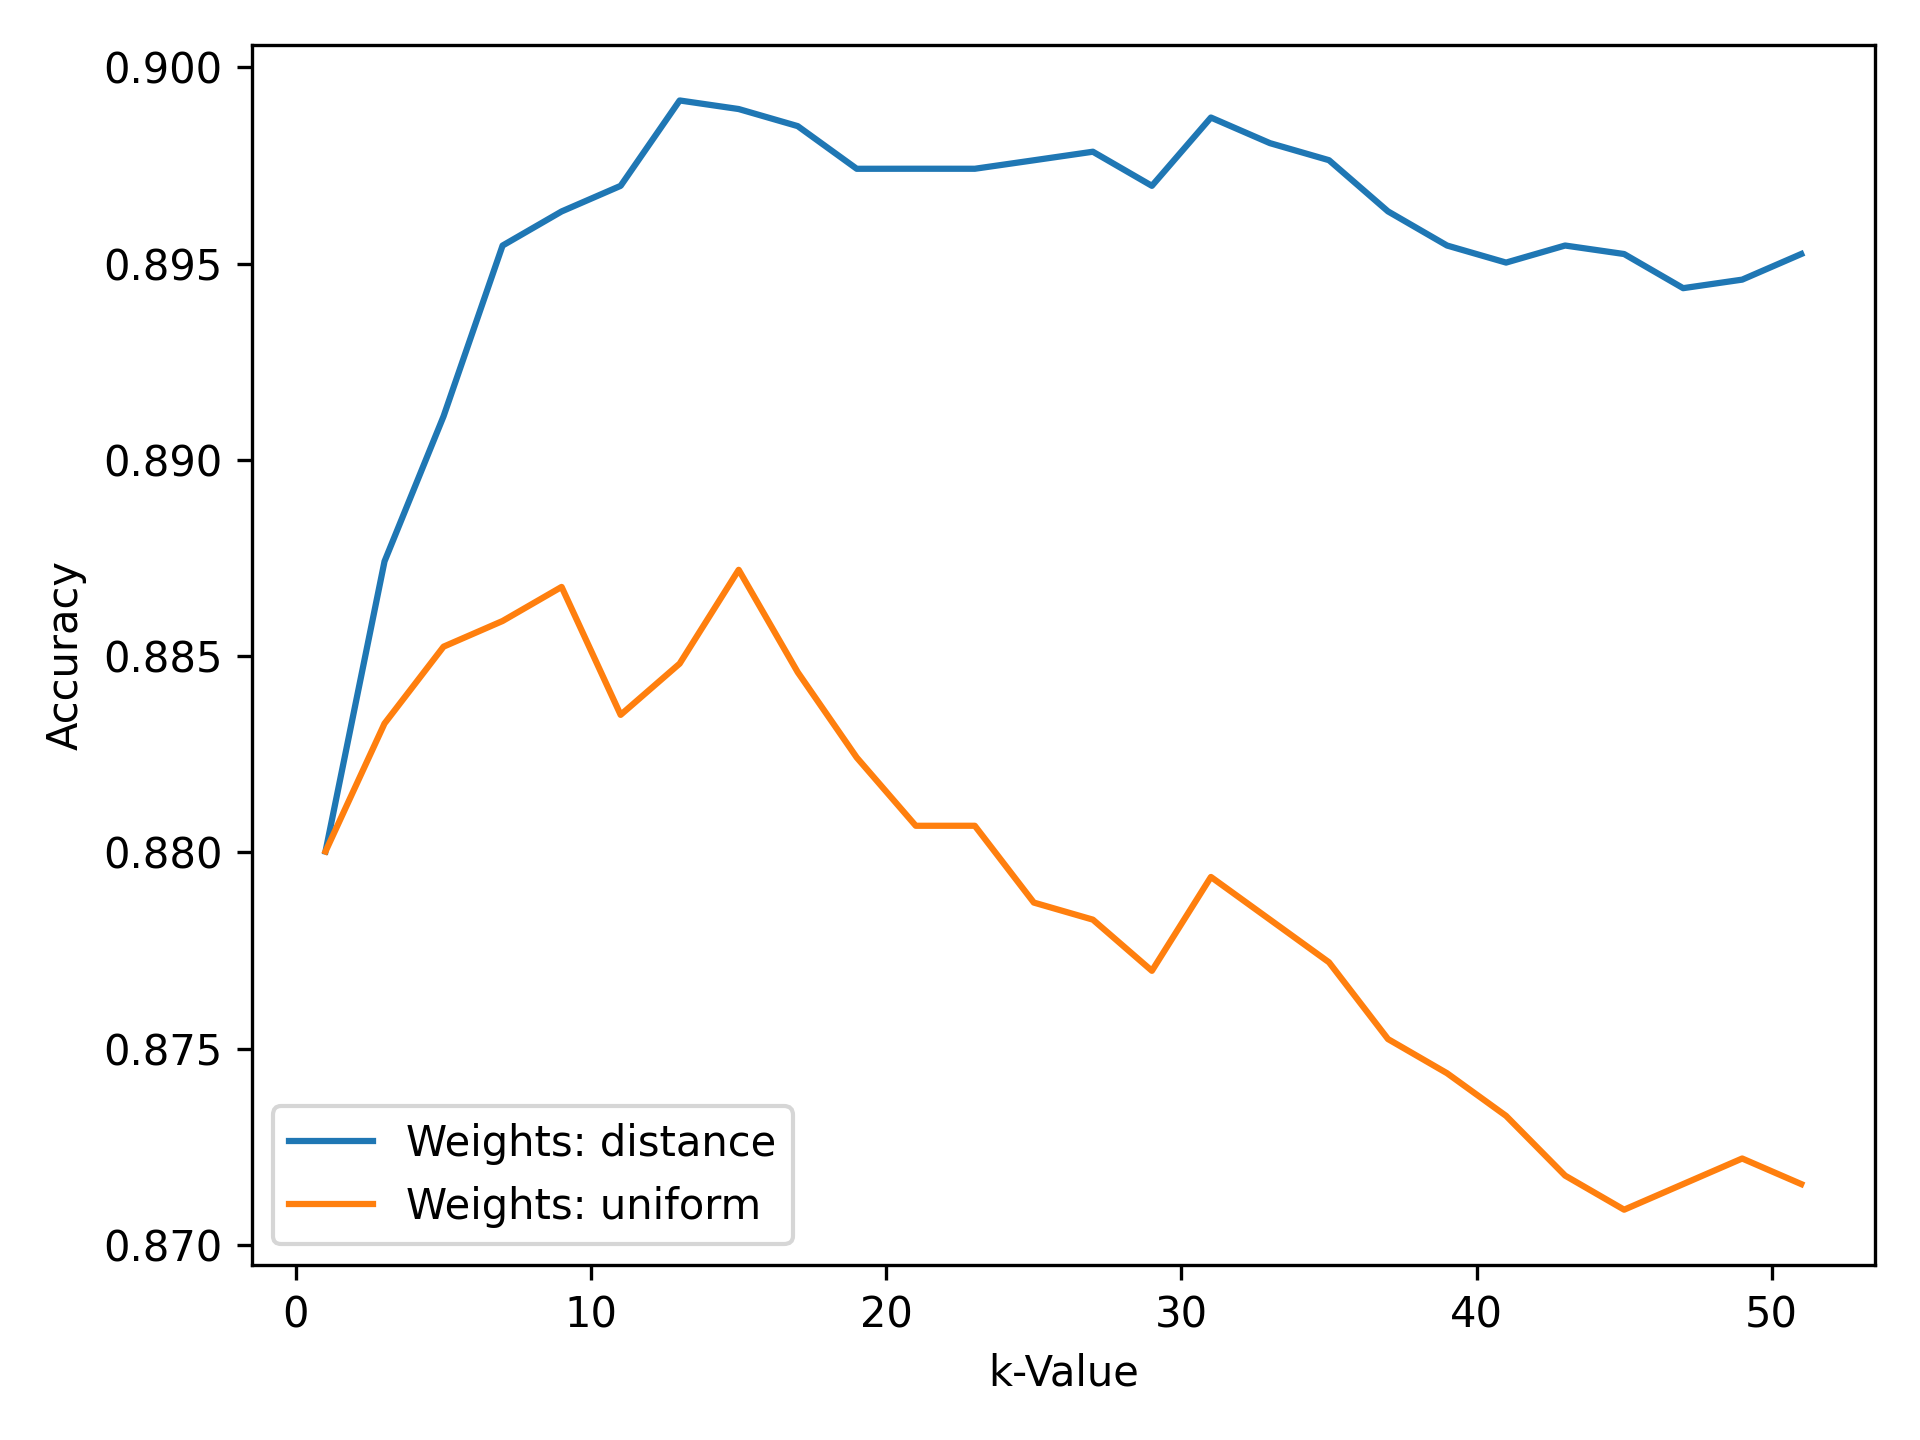
\includegraphics[width=1\textwidth]{exercise_1/paper/figures/spambase-accuracy-kNN.png}
                \caption{Accuracy}
                \label{fig:k-NN_spambase_accurracy}
            \end{subfigure}
            \begin{subfigure}[c]{0.45\textwidth}
                \centering
                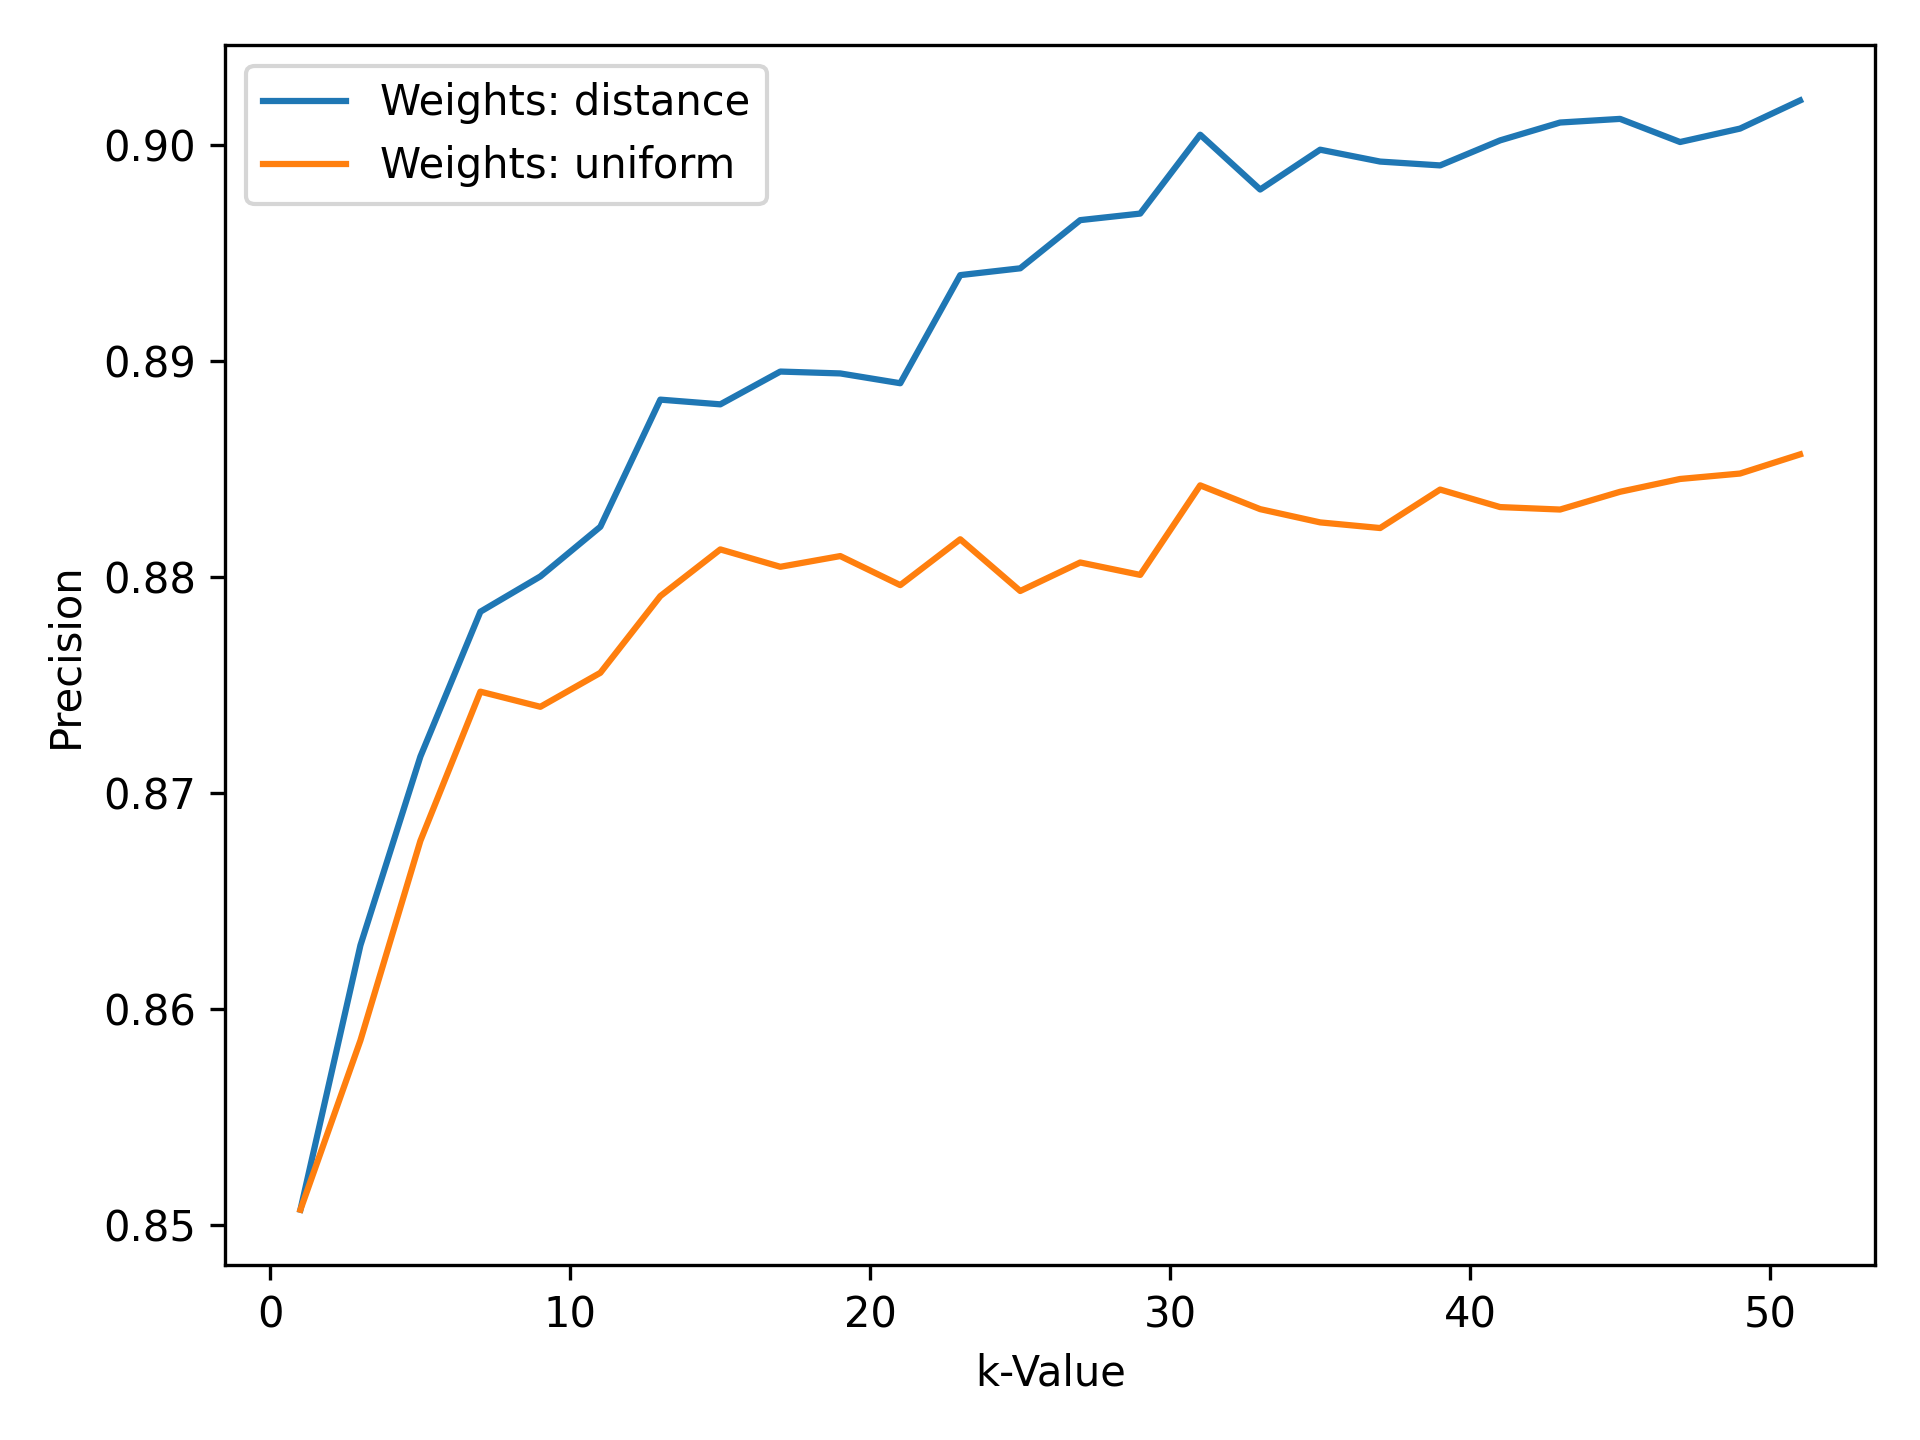
\includegraphics[width=1\textwidth]{exercise_1/paper/figures/spambase-precision-kNN.png}
                \caption{Precision}
                \label{fig:k-NN_spambase_precision}
            \end{subfigure}
            \caption{Performance measures for $k$-NN}
            \label{fig:k-NN_spambase}
        \end{figure}
    
        As the attributes have very different value ranges scaling was needed. We tried the min-max-scaler and the standard-scaler of scikit-learn and obtained better results by the latter, i.e.\ converting the mean of every attribute to 0 and the standard deviation to 1. Moreover, by using the distance as weight function the results could be improved a little bit more.
        
        For finding the optimal parameters to use in the $k$-NN algorithm we did a parameter search which returned $k=11$ as optimal value for the nearest neighbors algorithm. Additionally, we chose to use the Euclidean metric to calculate the distance between nodes. We tried using uniform weights for all neighbours, but came to the result that ranking them by their inverse distance gave us better results.
        
        We tested our classifier by comparing it to classifiers obtained by changing the parameters. As we would like to predict a binary attribute, we tried some different odd values for $k$ to ensure the optimality of this parameter. Furthermore, we tried to uniformly distribute the weights and using different distance metrices. But the classifier built with the parameters from the parameter search was the best resulting a score of $0.9227$. 
    
   % \subsection{Perceptron}
        %In the multilayer perceptron algorithm of scikit-learn we decided to vary the following parameters to optimize our classifier:
       % \begin{itemize}
          %  \item Maximum number of iterations
          %  \item Learning rate $alpha$
          %  \item solver = ['lbfgs', 'sgd', 'adam'] for optimizing the weights
       % \end{itemize}
       % We obtained the following: the maximum number of iterations does not have an impact on the classifier for big values, i.e. $1000$ iterations are enough. Moreover, with the default value for $alpha=0.0001$ we had a better classifier. Additionally, the stochastic gradient descent solver did better than the optimizer in the family of quasi-Newton methods 'lbfgs' and the default solver 'adam'. 
        
       % With these parameters we determined a classifier with an accuracy of $0.9392$. Hence, we could improve the classifier obtained by the $k$-NN algorithm. For us this means that the dataset is almost linearly separable.
        
    \subsection{Decision Tree}
        In Figure~\ref{fig:decision-tree_spambase} we compared the two criterion 'gini' and 'entropy' with respect to accuracy and precision. One can see that the performance highly depends on the maximum tree depth. For both performance measures the parameter setting with the best result is 'entropy' with a maximum tree depth of $8$. Limiting the length of a tree is very important, as seen in Figure~\ref{fig:decision-tree_spambase_precision}, as the precision is decreasing for growing tree depth. The reason for this is probably overfitting the decision tree to the training set. Moreover, our tests revealed using 'best' as splitter provides a bit better classifier than 'random'.
        
        \begin{figure}[h!]
            \centering
            \begin{subfigure}[c]{0.45\textwidth}
                \centering
                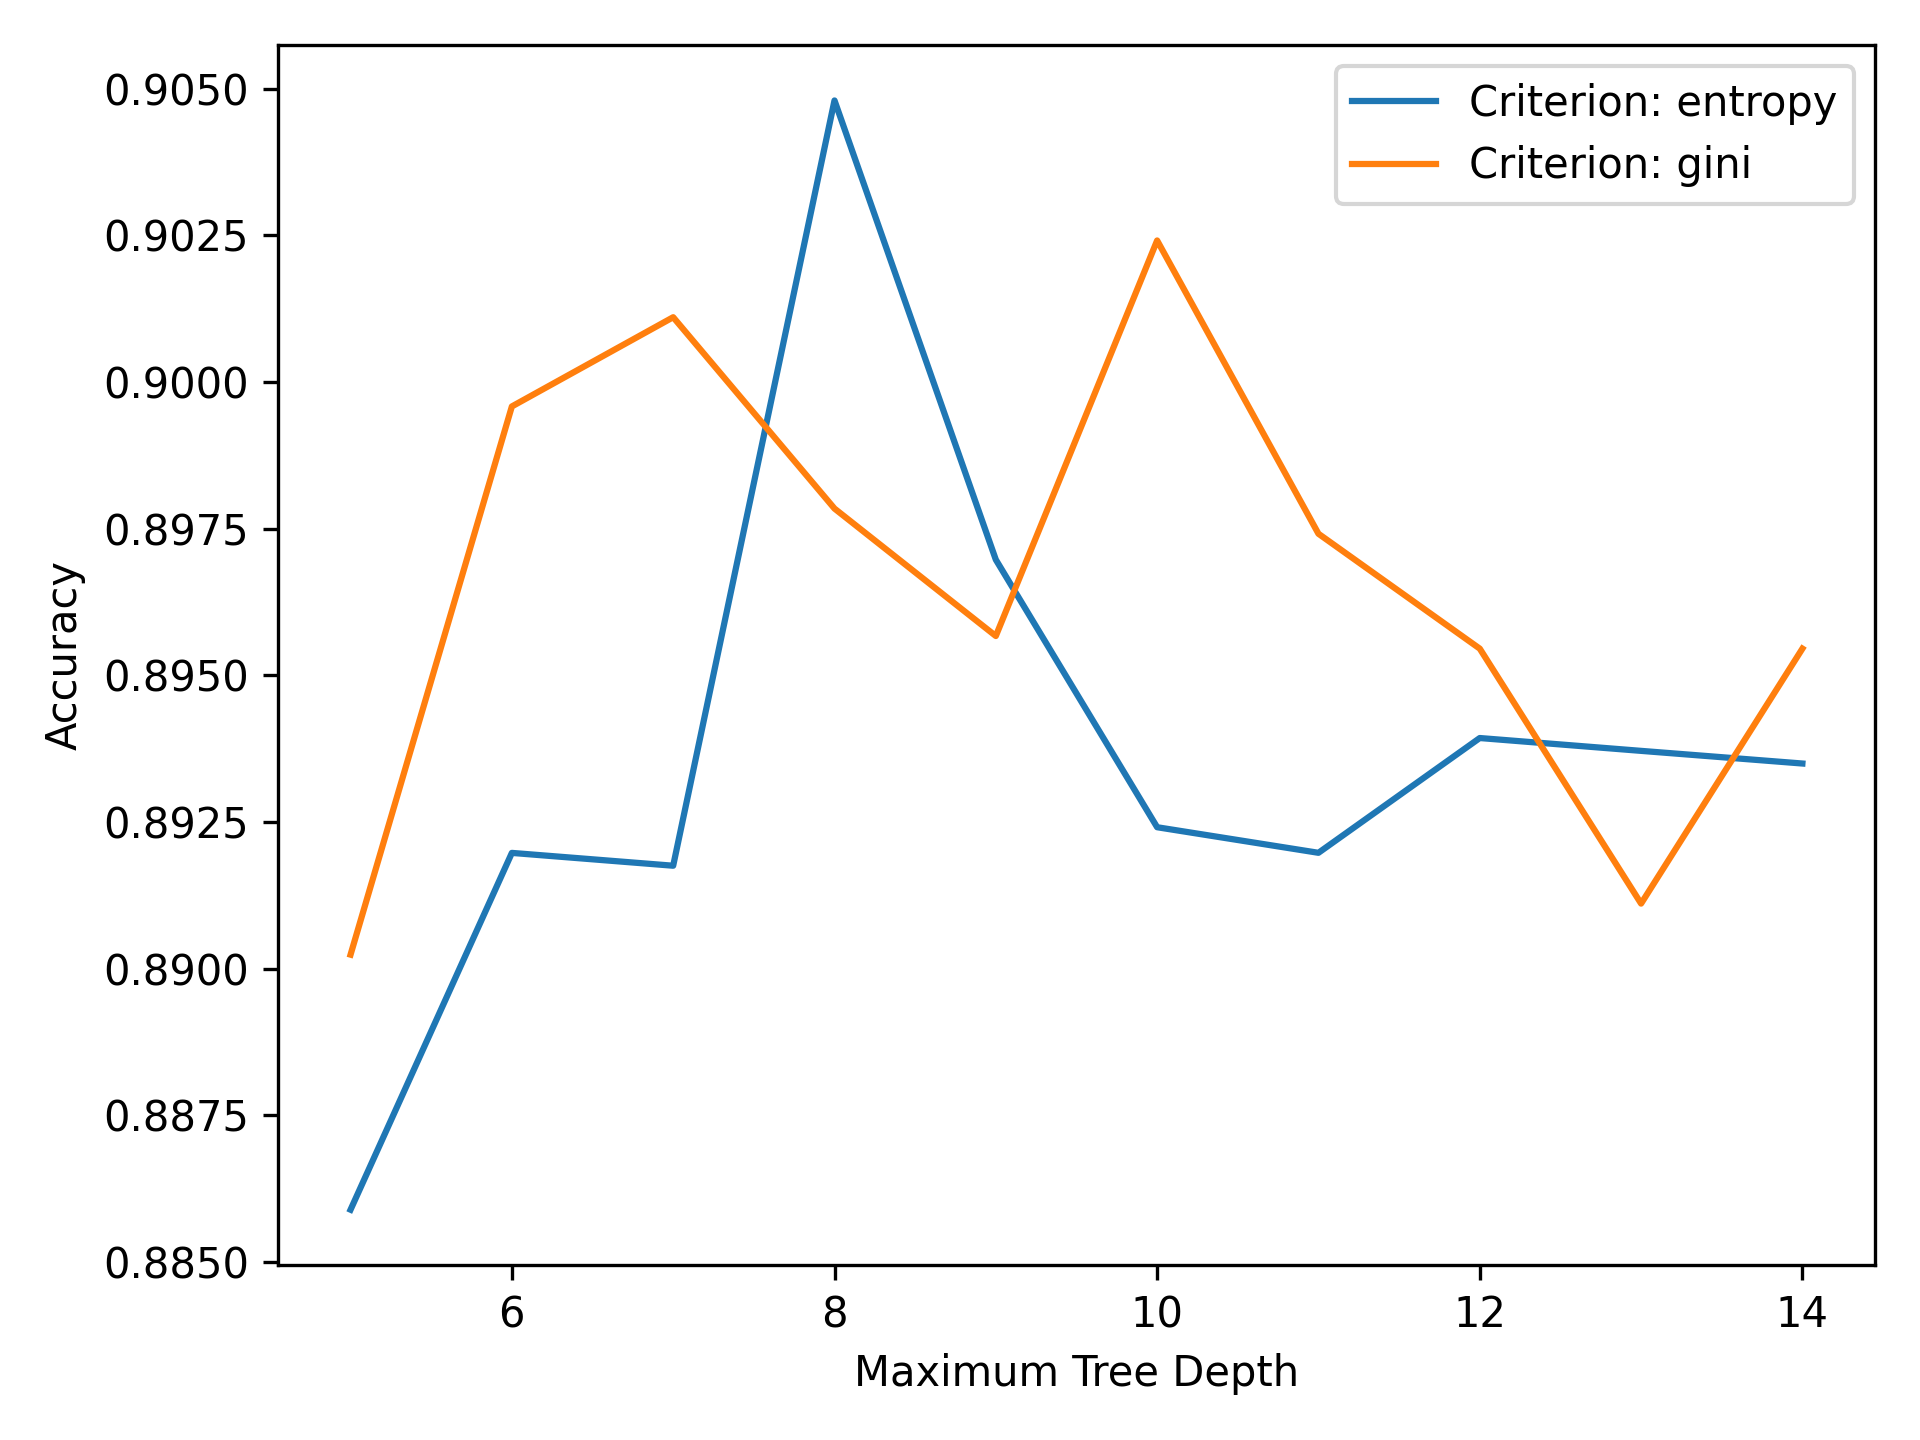
\includegraphics[width=1.1\textwidth]{exercise_1/paper/figures/spambase-accuracy-decision_tree.png}
                \caption{Accuracy}
                \label{fig:decision-tree_spambase_accurracy}
            \end{subfigure}
            \begin{subfigure}[c]{0.45\textwidth}
                \centering
                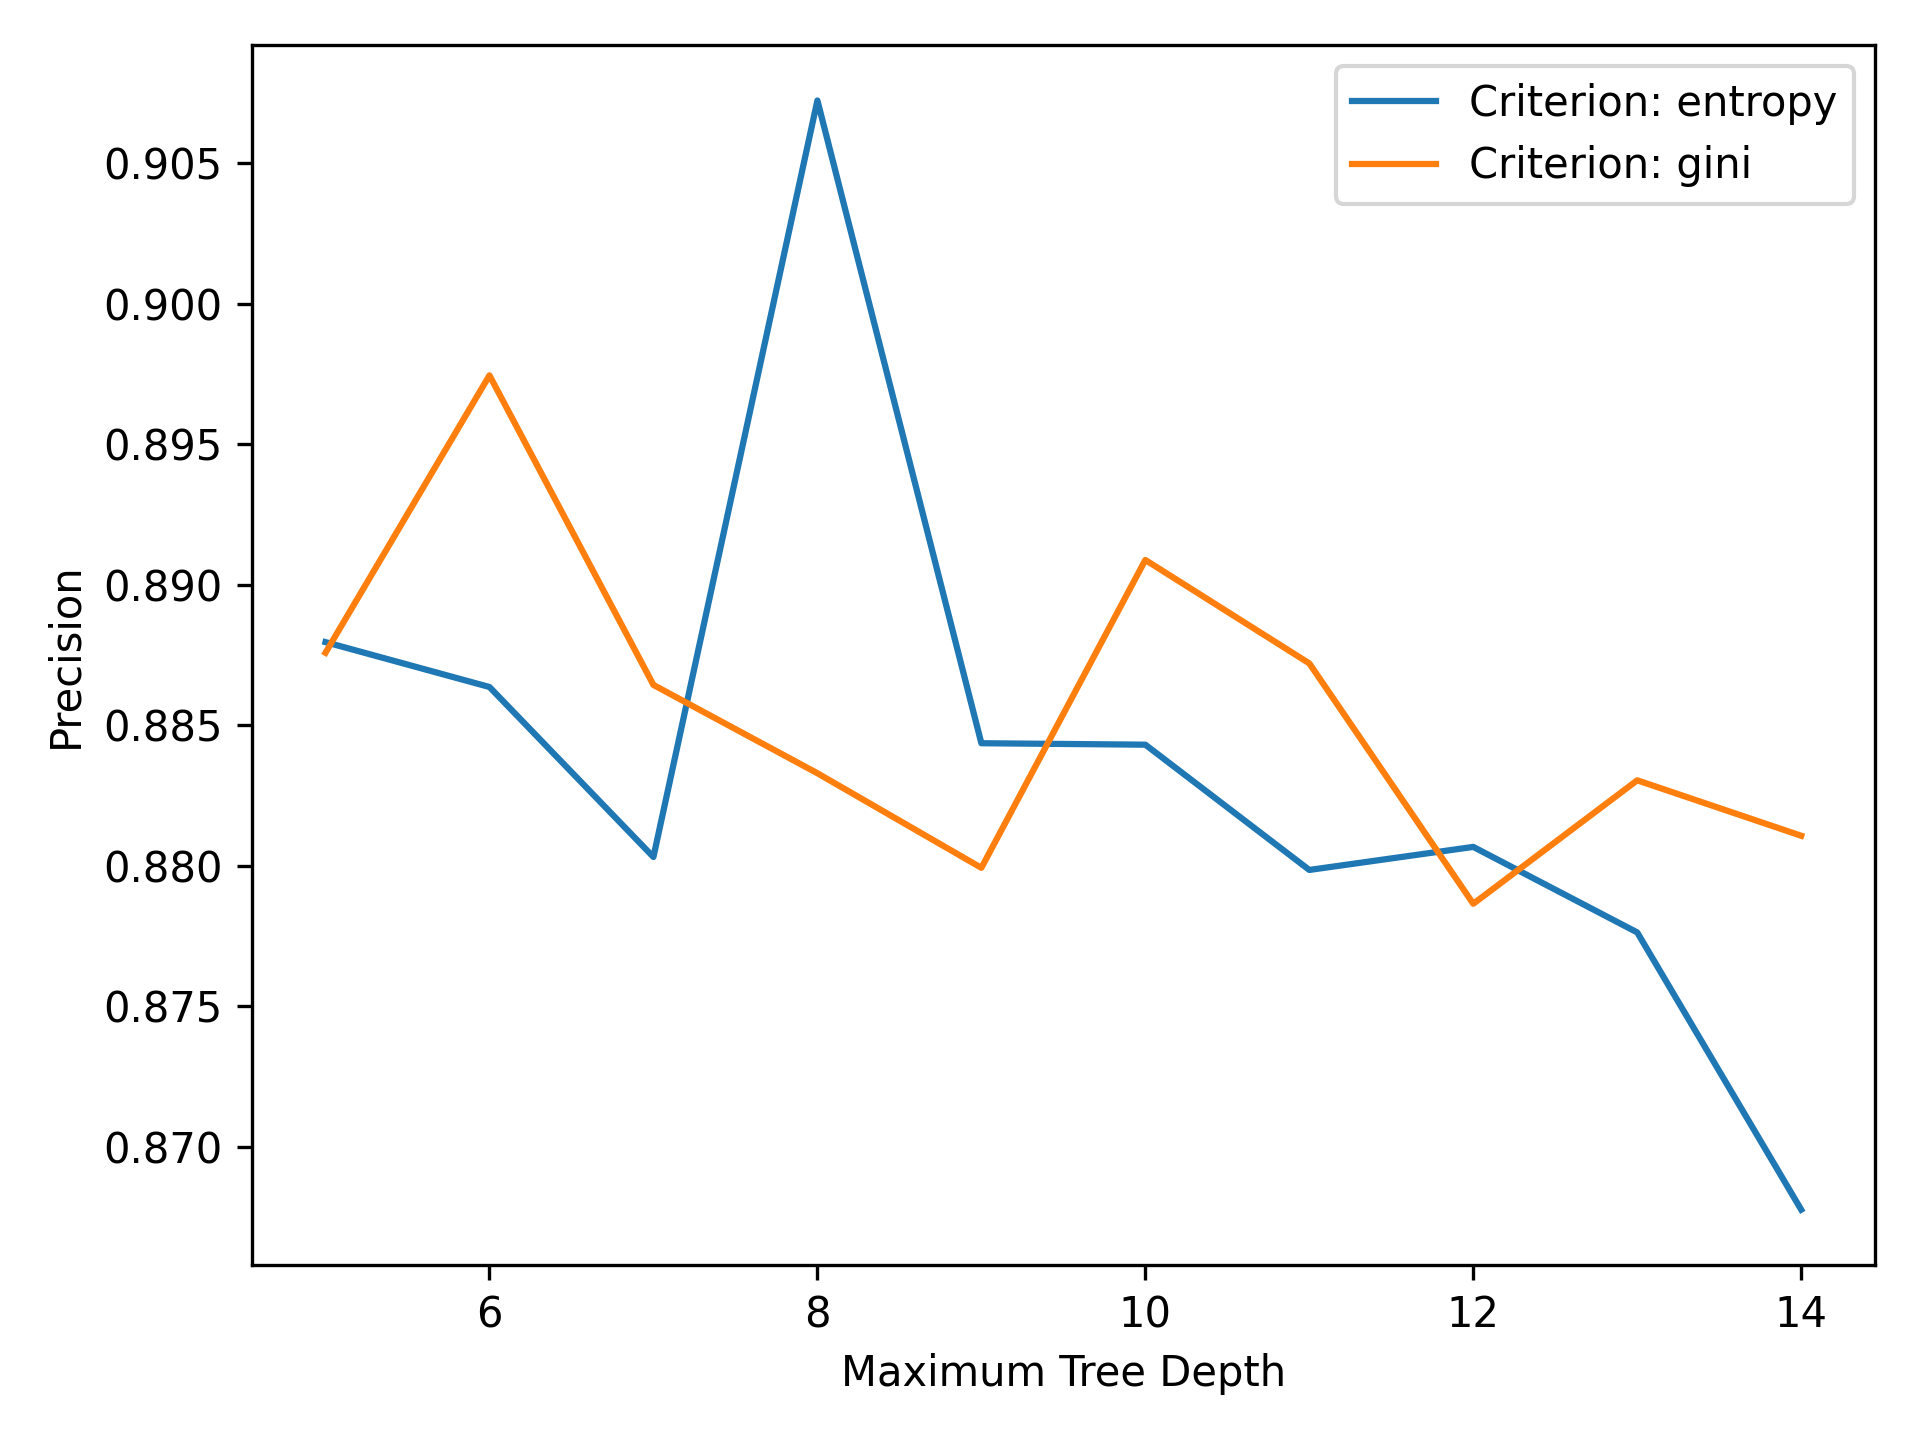
\includegraphics[width=1\textwidth]{exercise_1/paper/figures/spambase-precision-decision_tree.png}
                \caption{Precision}
                \label{fig:decision-tree_spambase_precision}
            \end{subfigure}
            \caption{Performance measures for decision tree }
            \label{fig:decision-tree_spambase}
        \end{figure}
        
        Using the best parameter settings we obtain a decision tree with an average accuracy of $0.91$, which is pretty good but still a bit worse than the previous classifier.

    \subsection{Random Forest}
        For this algorithm we once again did a parameter search to find optimal values for several parameters which were the following:
        \begin{itemize}
                \item Number of trees: $10\,000$
                \item Maximum depth of a tree: None
                \item Minimum number of samples required to split an internal node: $2$
                \item Minimum number of samples required to be at a leaf node: $1$
                \item Number of features to consider when looking for the best split: 'sqrt'
                \item Bootstrap samples are used when building tree: True
        \end{itemize}
        The random forest classifier learned with these parameter settings led to an average accuracy of $0.96$ via cross-validation. We also varied the parameter values but could not increase the performance.


\section{Credit Approval}
    This dataset is rather small compared to the previous dataset Spambase with only $690$ instances and $15$ attributes. It aims to predict whether a credit card application will be approved (true) or not (false) based on several categorical and continuous features. Figure~\ref{fig:credit-approval_classes_pie} shows the distribution of the classes in the given dataset. The two classes are not equally distributed, since there are more cases where the application is denied. 
    Although the proportion of True to False is not 1:1, there are still many cases where the credit card application is approved.
    \begin{figure}[h!]
        \centering
        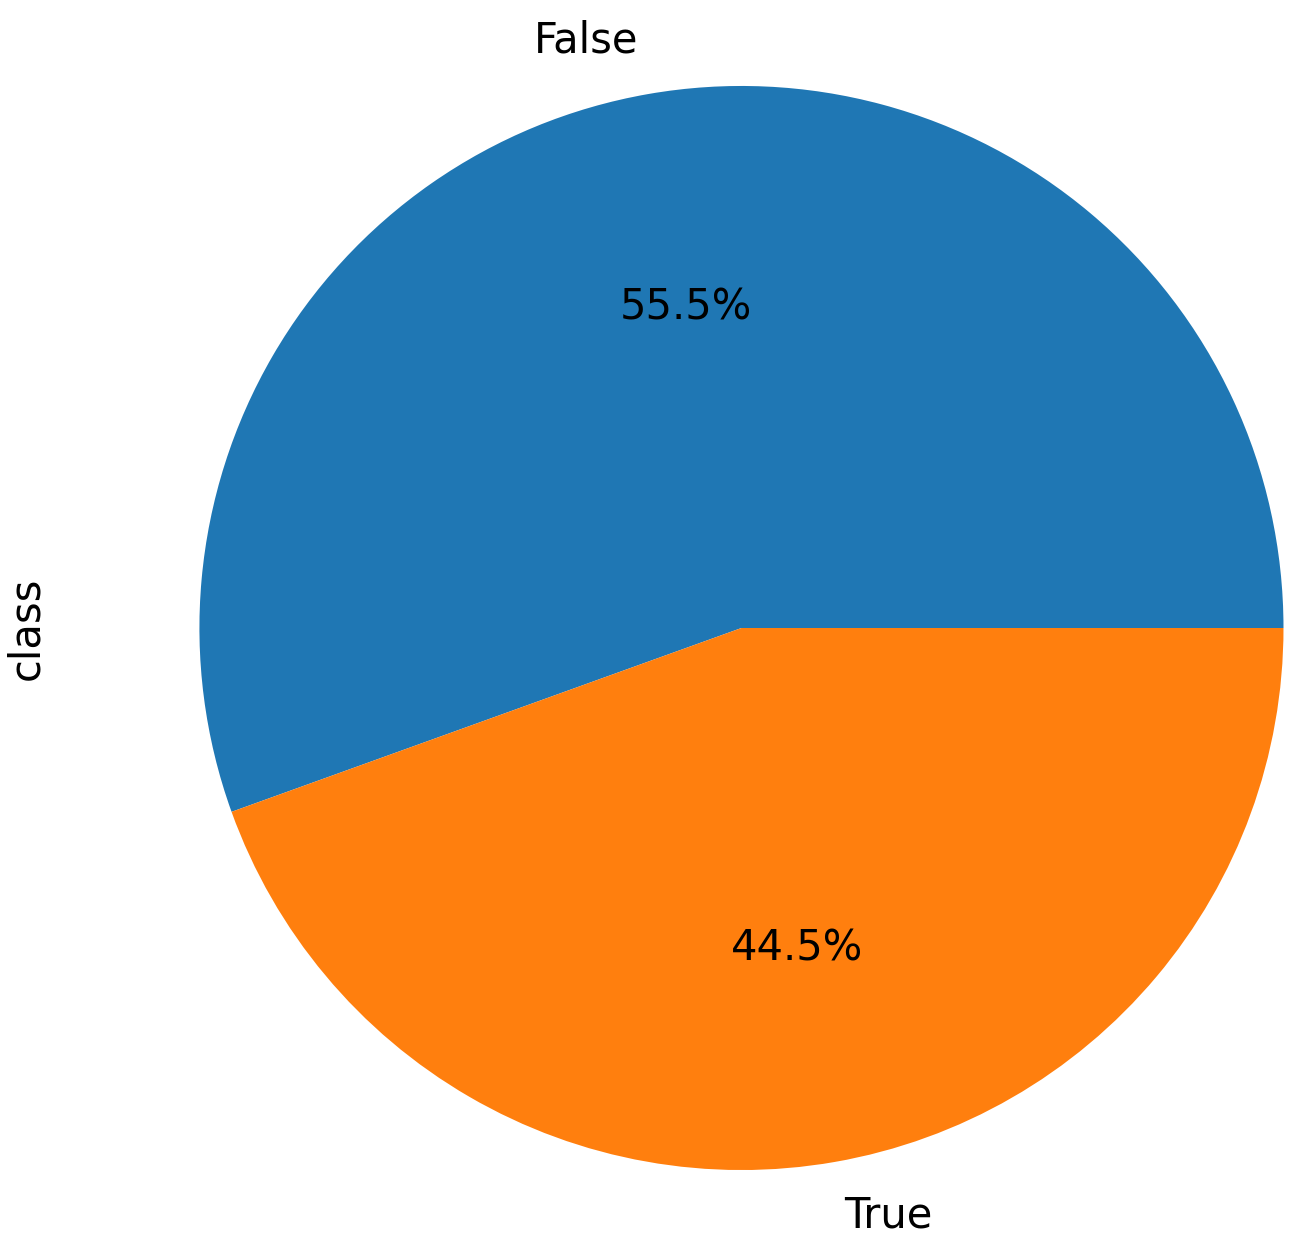
\includegraphics[width=0.5\textwidth]{exercise_1/paper/figures/credit_approval_pie.png}
        \caption{Class distribution}
        \label{fig:credit-approval_classes_pie}
    \end{figure}
    
    The Credit Approval dataset is interesting because of many factors. First, it has nominal as well as numeric attributes. The previous dataset 'Spambase' did not contain any nominal attributes except the predicted class. Figure~\ref{fig:credit-approval_attributes} shows some properties of the attributes in our dataset. A boxplot diagram of the value ranges of the numeric attributes can be seen in Figure~\ref{fig:credit-approval_numeric-attributes}, whereas the number of possible values of categorical attributes can be found in Figure~\ref{fig:credit-approval_categorical_attributes}. The diagrams show that the value ranges of both types of attributes are widely spread. We have numeric features with a range of $15$ but also one with a range of almost $100\,000$. But also the number of possible values for the nominal attributes varies between $2$ to $14$. 
    
    \begin{figure}[h!]
        \centering
        \begin{subfigure}[c]{0.4\textwidth}
            \centering
            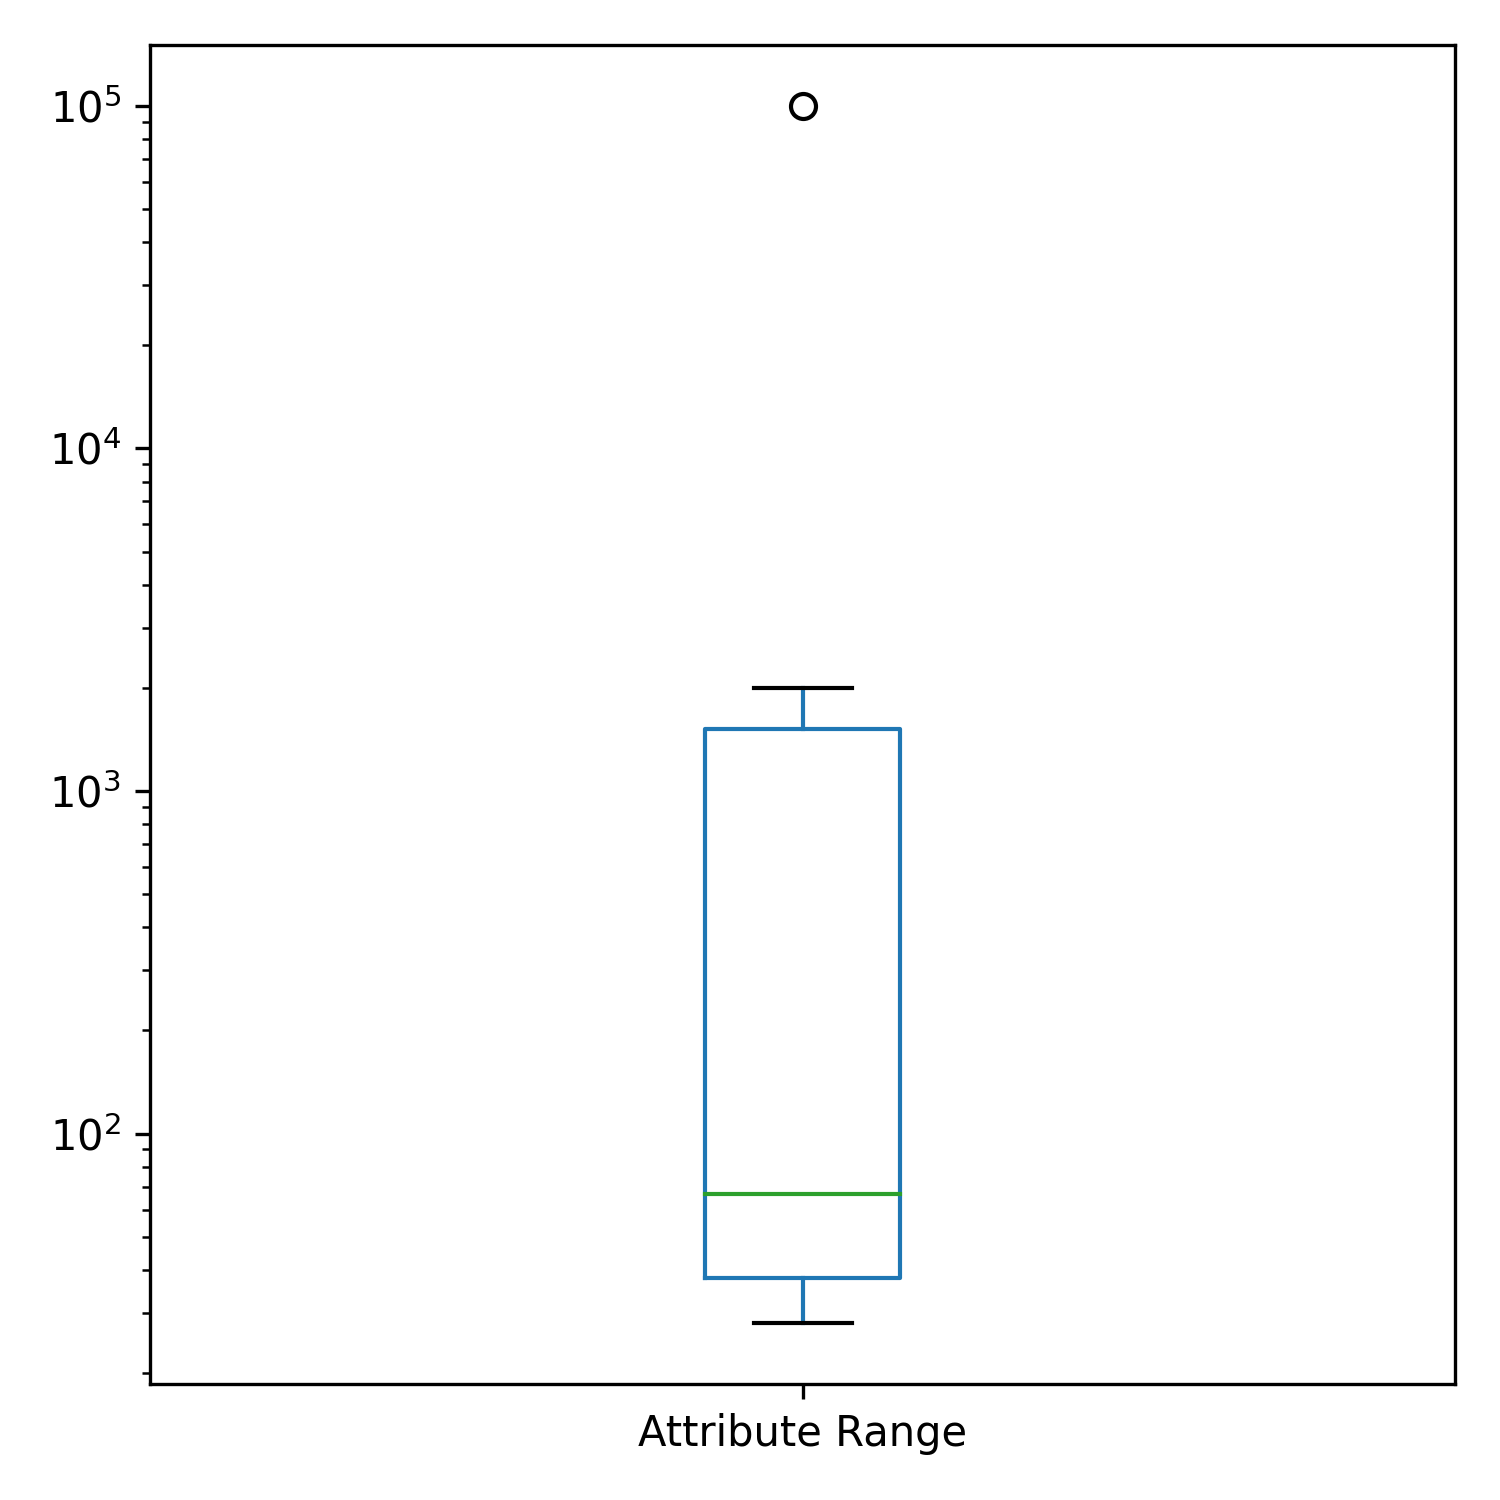
\includegraphics[width=1\textwidth]{exercise_1/paper/figures/credit_approval_continous_range_plot.png}
            \caption{Boxplot of the values ranges of the numeric attributes}
            \label{fig:credit-approval_numeric-attributes}
        \end{subfigure}
        \begin{subfigure}[c]{0.5\textwidth}
            \centering
            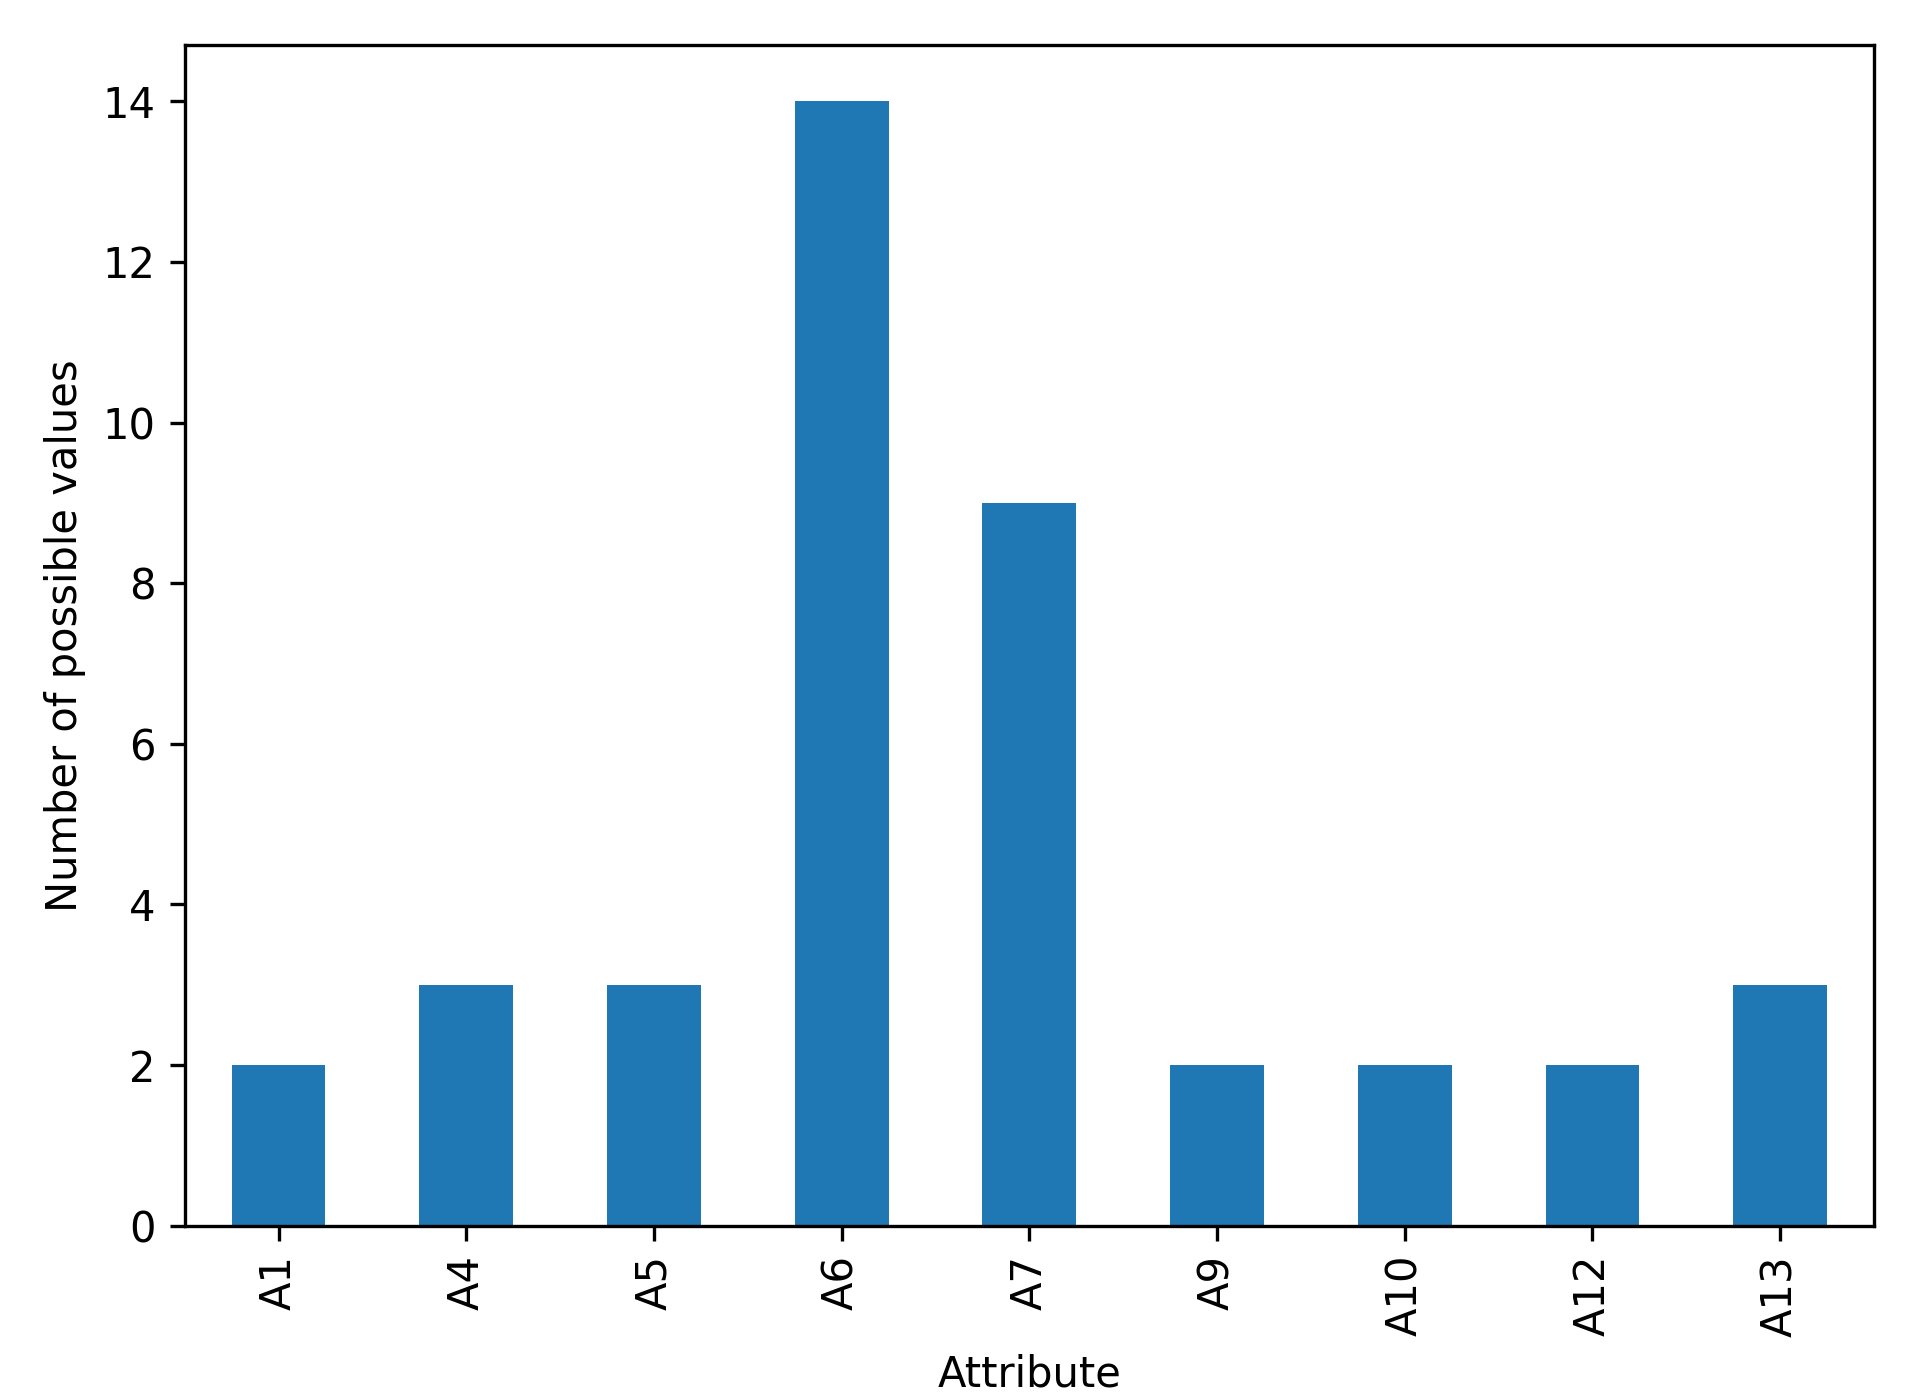
\includegraphics[width=1.1\textwidth]{exercise_1/paper/figures/credit_approval_categories_bar.png}
            \caption{Number of possible values for categorical attributes}
            \label{fig:credit-approval_categorical_attributes}
        \end{subfigure}
        \caption{Features of Credit Approval dataset}
        \label{fig:credit-approval_attributes}
    \end{figure}
    
    Moreover, the Credit Approval dataset also contains missing values. About $5\%$ of the instances have some missing values. We decided to impute the values in different ways and see how it affects the performance of the classifiers. We univariately estimated the values by the mean, median resp. the most frequent value. As the true und false classes were roughly the same size we chose to only look at the accuracy for this dataset.
    
    \subsection{$k$-NN}
        For $k$-NN the first question was obviously how to translate the nominal values to numeric values in order to measure a distance. For this we decided for binary nominal attributes to assign either $0$ or $1$. For the remaining categorical attributes we used one hot encoding. 
        Next, we normalised the numeric values via the integrated min-max resp.\ normalised scaler and run $k$-NN algorithm.
        
        \begin{figure}[h!]
            \centering
            \begin{subfigure}[c]{0.45\textwidth}
                \centering
                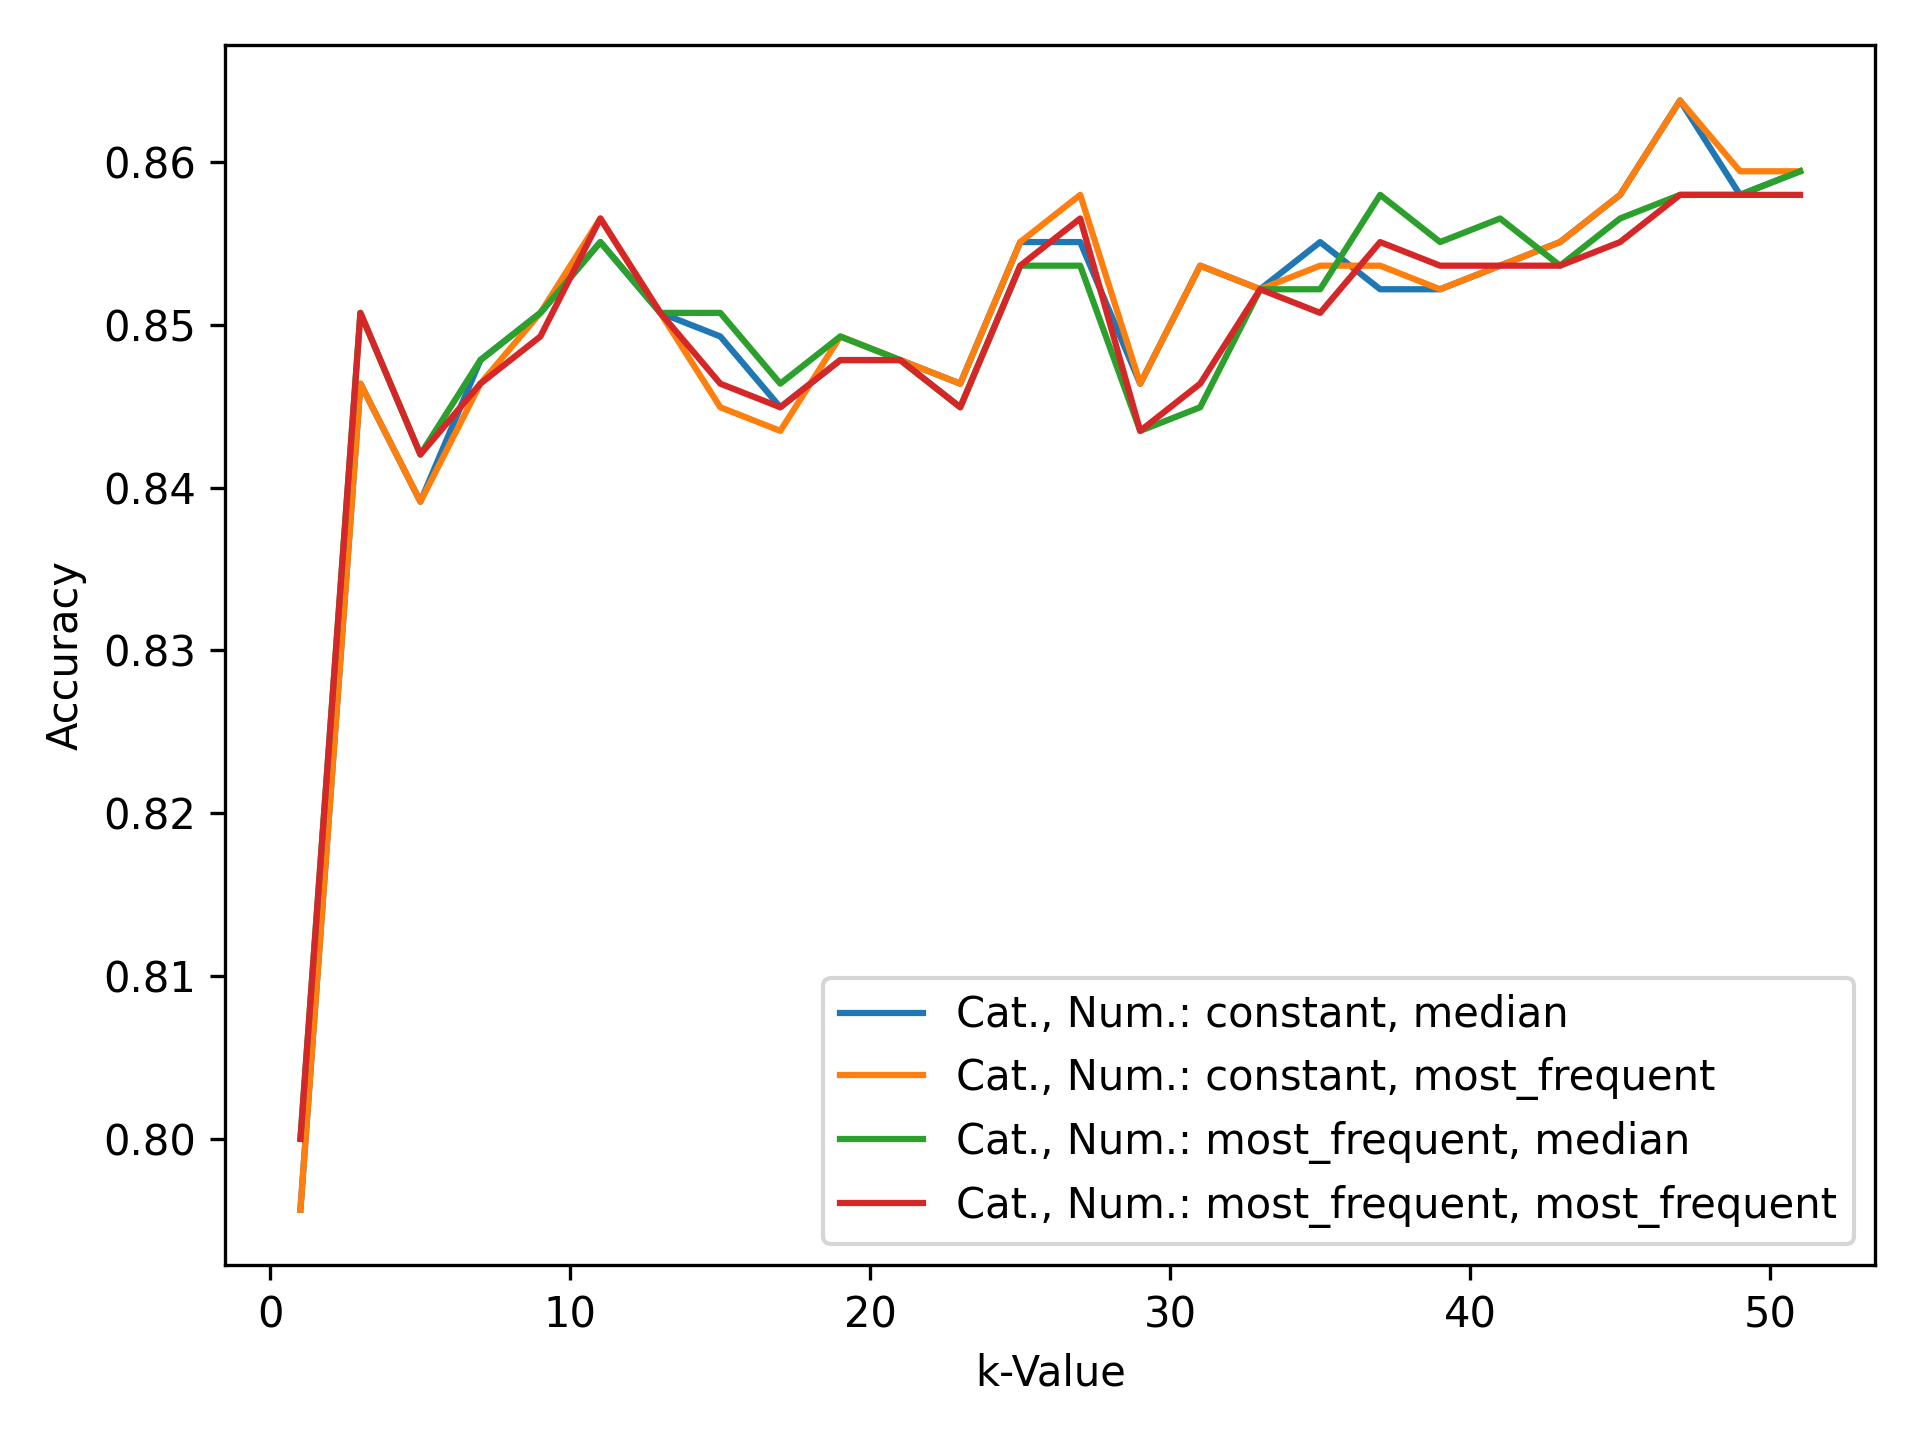
\includegraphics[width=1\textwidth]{exercise_1/paper/figures/credit-approval-accuracy-kNN_uniform.png}
                \caption{Uniform weights}
                \label{fig:k-NN_credit-approval_uniform}
            \end{subfigure}
            \begin{subfigure}[c]{0.45\textwidth}
                \centering
                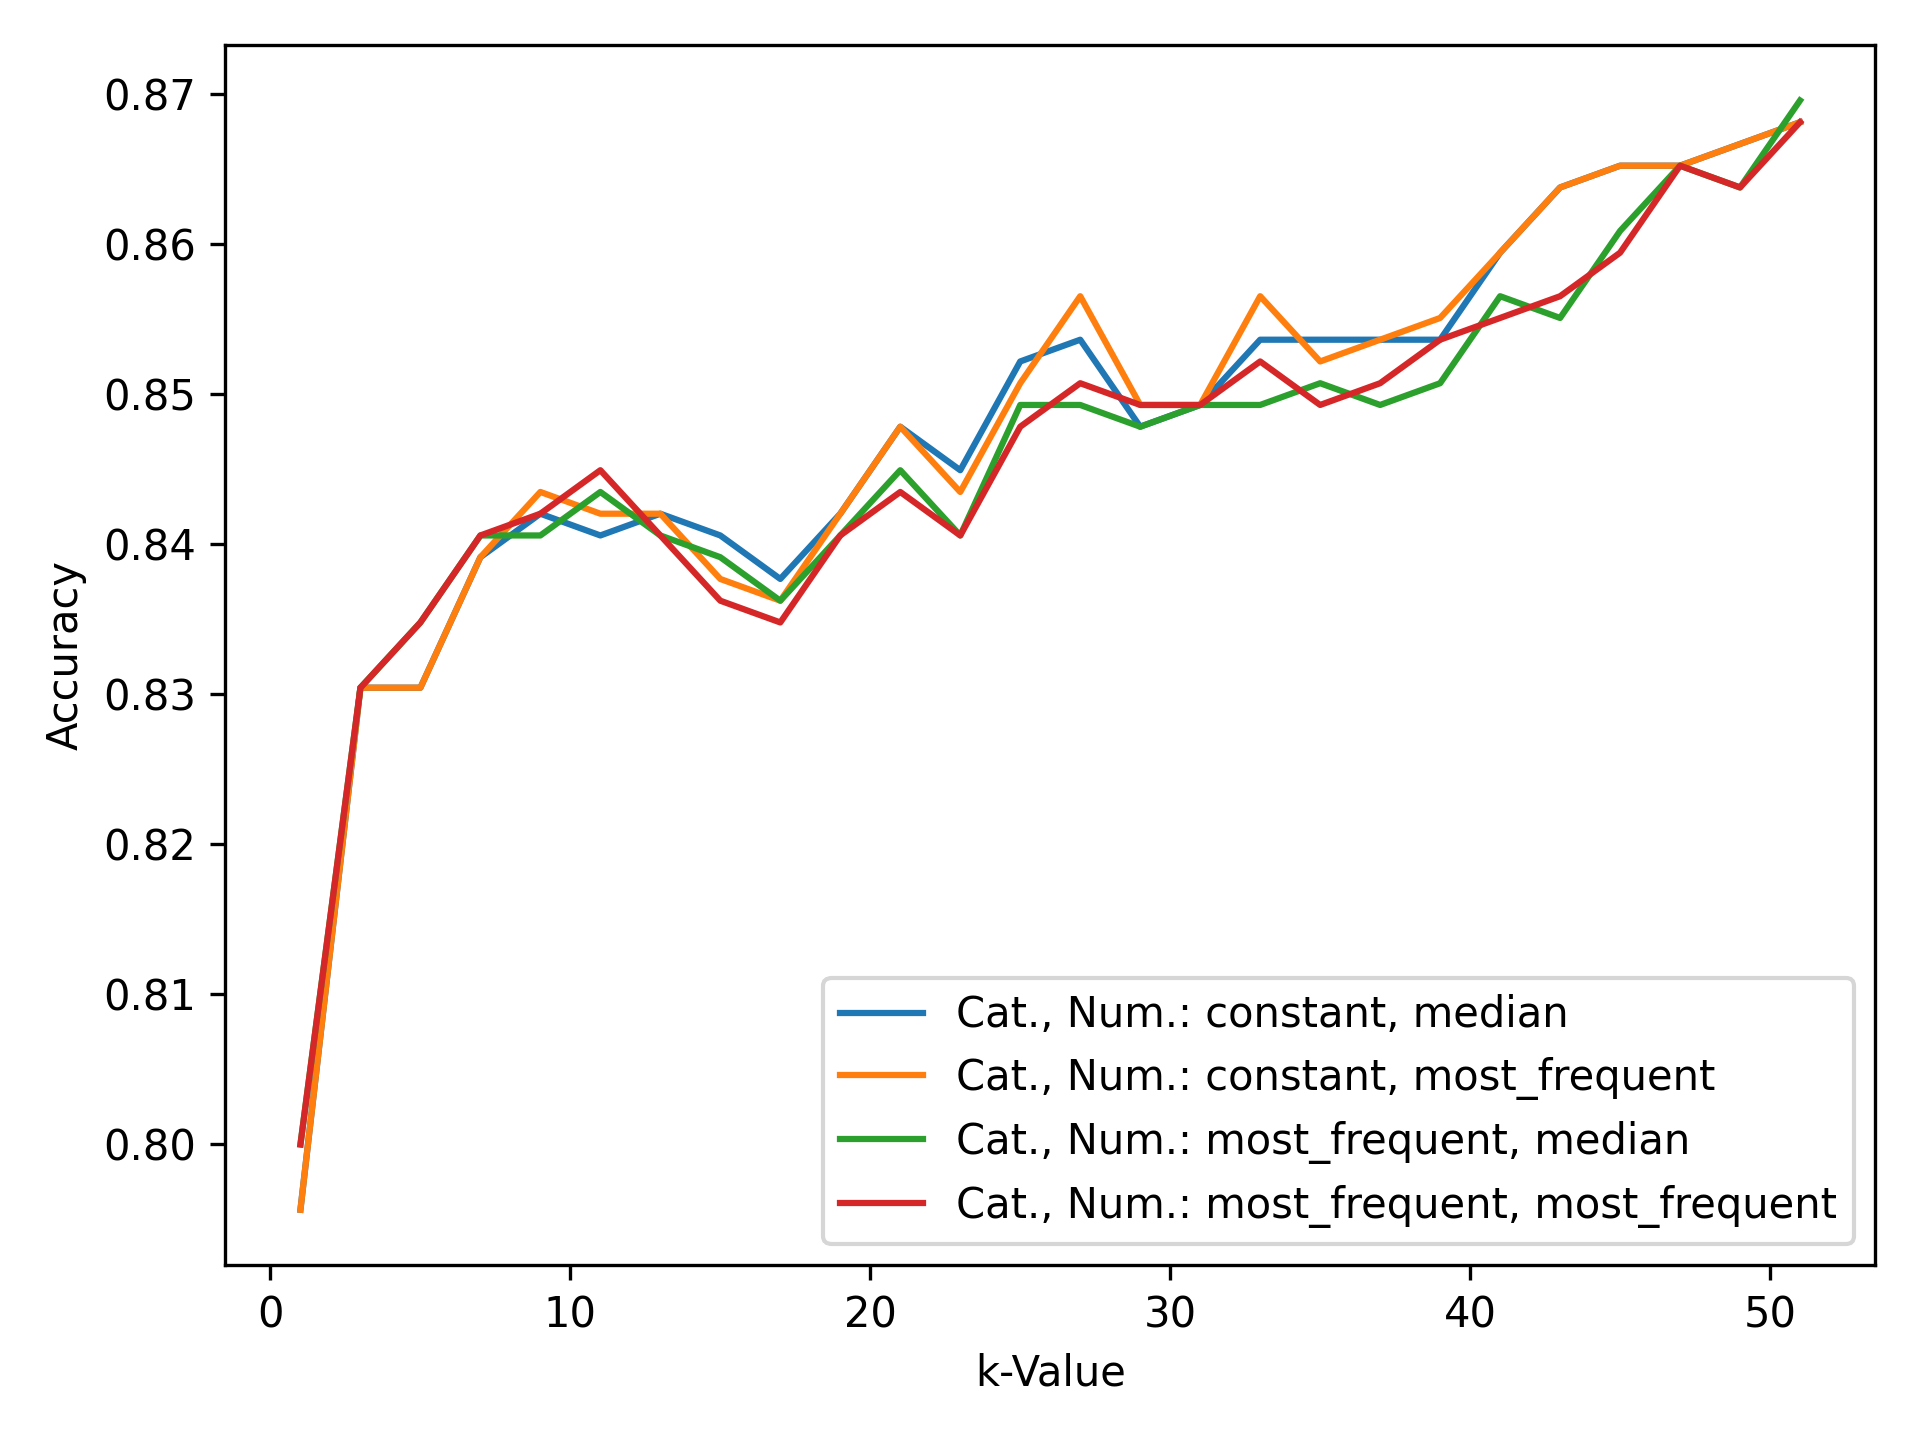
\includegraphics[width=1\textwidth]{exercise_1/paper/figures/credit-approval-accuracy-kNN_distance.png}
                \caption{Distance-based weights}
                \label{fig:k-NN_credit-approval_distance}
            \end{subfigure}
            \caption{Comparision of imputation methods}
            \label{fig:k-NN_credit-approval}
        \end{figure}
        
        For missing values we had different approaches which can be seen in Figure~\ref{fig:k-NN_credit-approval}. This includes substituting missing values of a categorical attribute with the most frequent one or with a constant, which stands for a missing value, i.e. we are adding a new value to the attribute. Missing values of numeric attributes are replaced with the median, the mean or the most frequent one. Our tests showed that using the median or the mean value makes no difference. This is the reason why we omitted the approach with the mean value.
        
        As one can see in Figure~\ref{fig:k-NN_credit-approval} the differences between the different imputation methods were negligible. One reason for this is probably the comparatively small amount of missing values in the dataset.
        It is also apparent from the graph that the uniform weights performed better than the distance-based weights for lower $k$ values. The reason for higher $k$ values still having a good performance could be that instances that are classified the same are grouped together rather closely.
        
        Again, we did a parameter search to determine the best values, which returned $k=35$. By using a simple imputation which replaces each missing value by the median, we got an accuracy of 
        $0.849$ for this $k$ value. Using the most frequent value in the imputation led to a minimal drop of accuracy to $0.843$. Without scaling the accuracy dropped to $0.67$. Additionally, we tried different values for $k$ which led to worse results. Using min-max scaling instead of the normalised scaling had no impact on the results.
        
        We also tried to impute the missing values by simply assigning the most frequent value of the attribute or inserting a new "missing" category and afterwards one hot encoding it. This led to an optimal parameter $k=37$ and the best accuracy of $0.855$. Changing between uniform weight and weights based on distance made a negligible difference.
        
   % \subsection{Multilayer Perceptron}
      % Perceptron with the maximal number of iterations being $100000$ and $\alpha=10^{-5}$ led to an accuracy of $0.8$.
       %\todo[inline]{other values}
        
    \subsection{Decision Tree}
        As one can see the imputation method had greater influence on the decision tree model, than the $k$-NN model. This could be due to the fact that while a single wrongly approximated attribute does not greatly change the distance between two instances, it could lead to the instance being put down a whole other path on the decision tree and therefore lead to a wrong result.  
        
        \begin{figure}[h!]
            \centering
            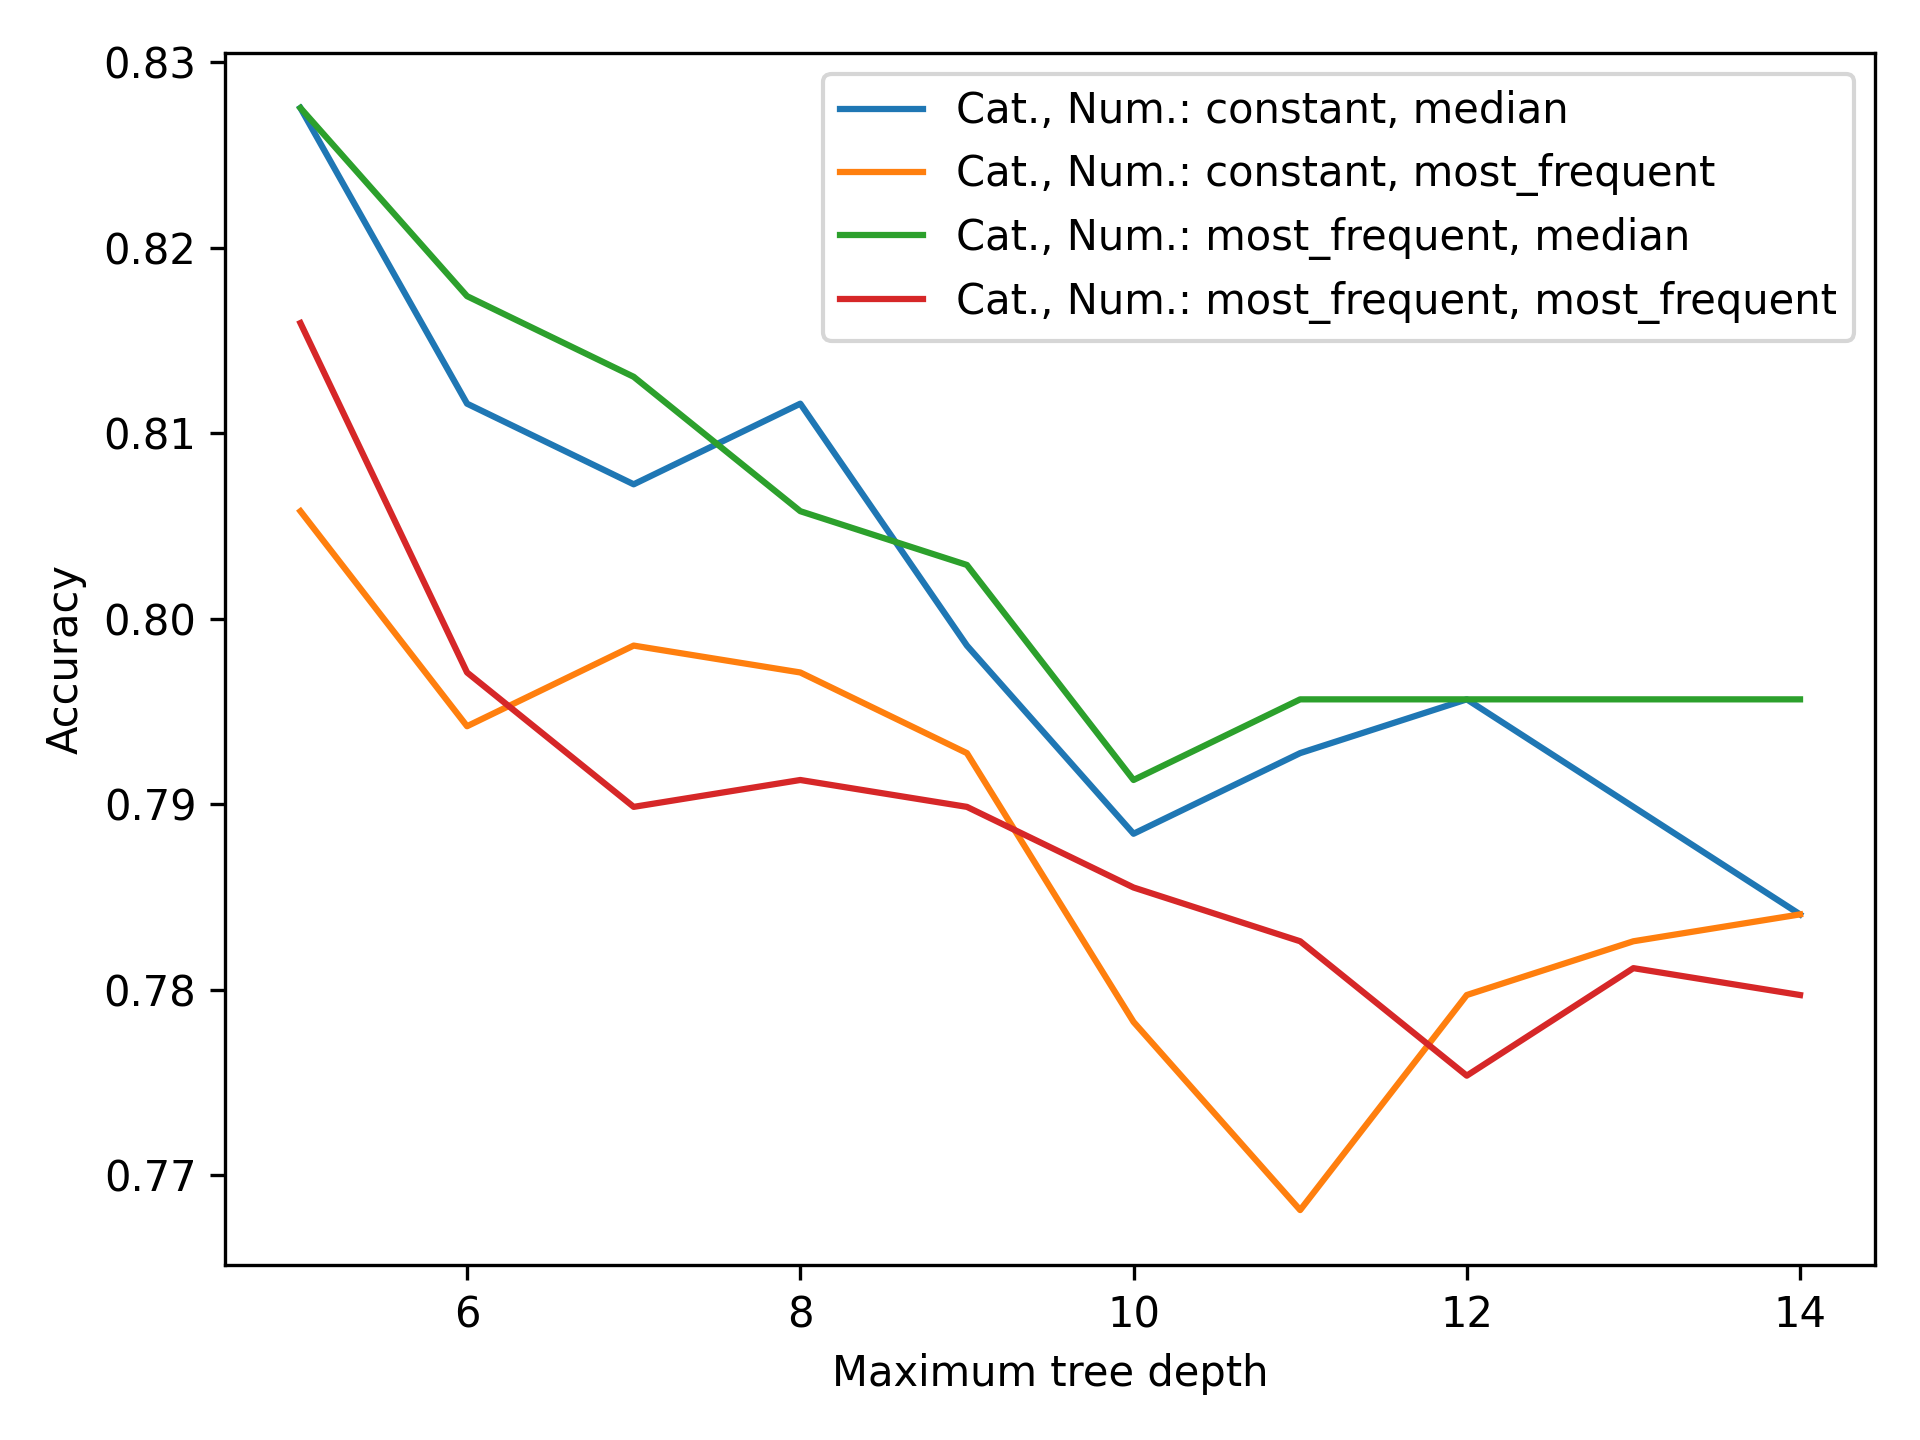
\includegraphics[width=0.6\textwidth]{exercise_1/paper/figures/credit-approval-accuracy-decision_tree.png}
            \caption{Influence of imputation on accuracy}
            \label{fig:credit-approval_decision_tree}
        \end{figure}
        
        In order to determine which parameters would lead to an optimal decision tree we once again did a parameter search, which gave us the following parameter settings, which are consistent with the figures above. Use 'gini' to measure the quality of a split, limit the maximum tree depth to $5$ and 'random' as strategy to choose the split at each node. Using these parameters the learned classifier had an accuracy of $0.832$. 
        
    \subsection{Random Forest}
        Like for the previous classifiers we evaluated different parameter settings and then confirmed the obtained results with a parameter search. We obtained the following optimised parameter settings:
        \begin{itemize}
            \item Number of trees: $10\,000$
            \item Maximum depth of a tree: $50$
            \item Minimum number of samples required to split an internal node: $5$
            \item Minimum number of samples required to be at a leaf node: $1$
            \item Bootstrap samples are used when building tree: True
        \end{itemize}
        
        The corresponding built classifier led to an accuracy of $0.862$. This was the best value which we could achieve as we also tested it with other parameter settings but could not improve this. Comparing this result with the classifiers of the previous of this dataset this has a slightly better accuracy, hence slightly better.
        
        %parameter search: parameters
            %'randomforestclassifier__max_features': 'sqrt', 'randomforestclassifier__class_weight': 'balanced_subsample'

\section{Conclusions}
    Summing up we can say, that in general there is no algorithm building a classifier that could predict the respective attribute perfectly in each case for every dataset. In particular, there is not even an algorithm that is optimal for each dataset as we could see from the results.
    
    Although the classifiers returned from the random forest algorithm were mostly pretty good and in many cases even the best, it was outperformed by $k$-NN in the Breast Cancer dataset. Although $k$-NN had a perfect result for the Breast Cancer dataset in the public split of Kaggle, it failed at classifying the more complex dataset Amazon.
    
    $k$-NN and decision tree where both rather sensitive on big changes of the parameters for the algorithm, however random forest was not. The reason for this is probably that the random forest algorithm builds its classifier by taking the average of a specified of number decision trees.
    
    The longest runtime of all algorithms had random forest for all datasets, especially for the Amazon review dataset. The runtime of this algorithm increased in particular for huge tree sizes, which however generally performed better on this dataset. This proved very problematic for the parameter searches, which could not be performed within a reasonable time frame for higher number of trees. Figure~\ref{fig:runtime-comparison} shows the runtime in seconds of the random forest algorithm for constructing a classifier using $1\,000$ decision trees. It shows that the runtime also depends on the number of samples and number of features, not only on the parameters.
    
    \begin{figure}[h!]
            \centering
            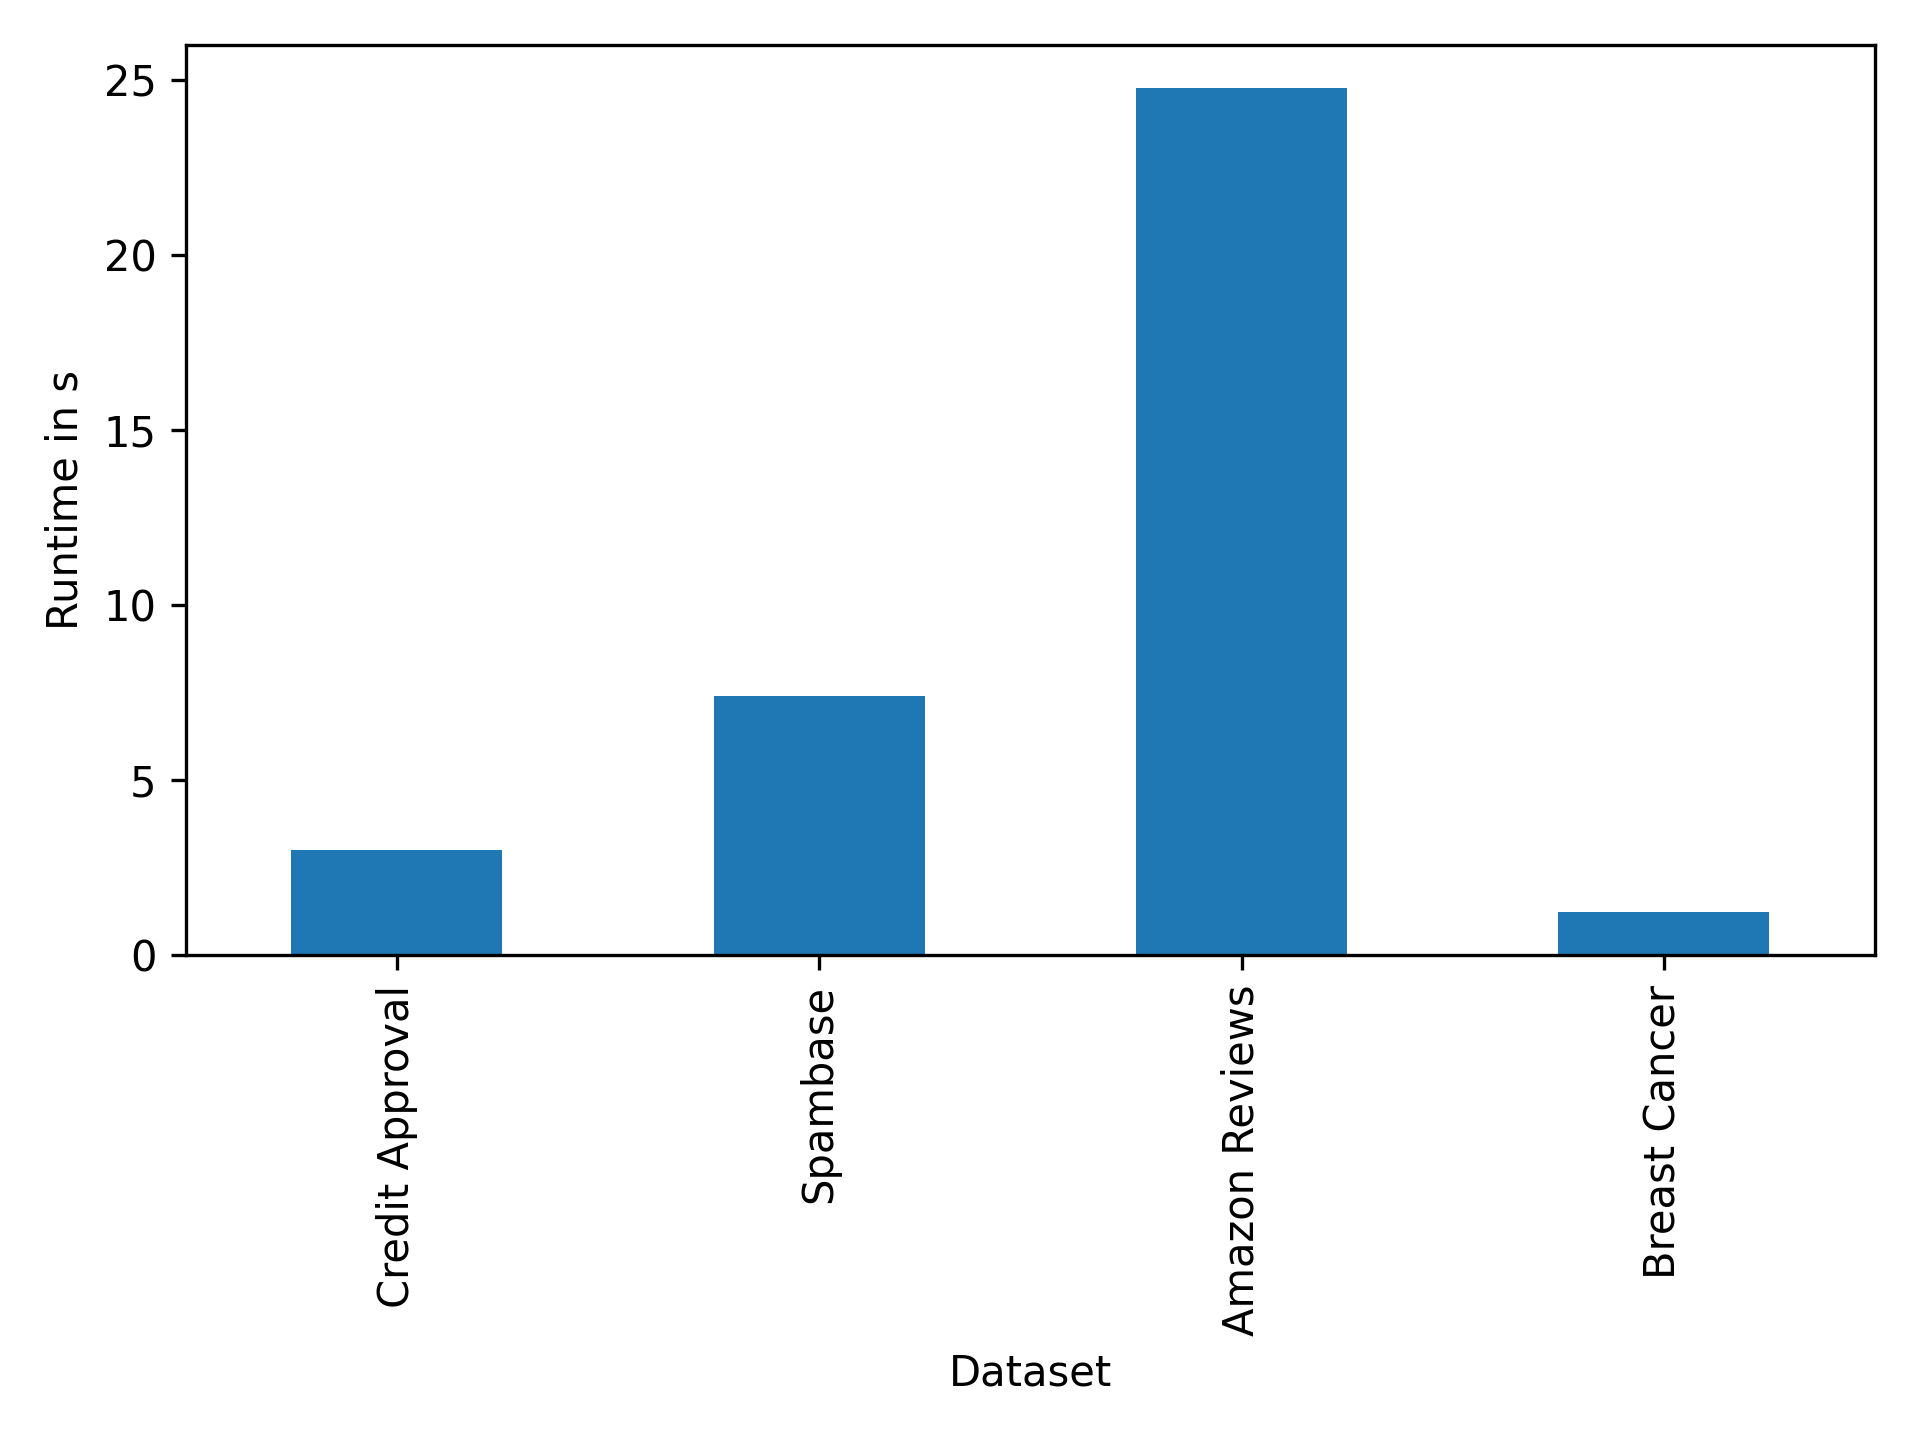
\includegraphics[width=0.55\textwidth]{exercise_1/paper/figures/runtime_comparison.png}
            \caption{Runtime comparison of different classification algorithms}
            \label{fig:runtime-comparison}
    \end{figure}

\end{document}